% Author: Alfredo Sánchez Alberca (asalber@ceu.es)
% !TEX program: xelatex
%----------------------------------------------------------------------------------------
%    DOCUMENT CLASS
%----------------------------------------------------------------------------------------

\documentclass[11pt,a4paper,openright]{book}
%----------------------------------------------------------------------------------------
%	PACKAGES AND OTHER DOCUMENT CONFIGURATIONS
%----------------------------------------------------------------------------------------

% Language settings
\usepackage{polyglossia}
\setdefaultlanguage{english}

% Margins and layout
\usepackage[top=3cm, bottom=3cm, left=2.54cm, right=2.54cm]{geometry}

% Font settings
\usepackage{fontspec}
\usepackage{unicode-math}
\setmainfont[Ligatures=TeX]{TeX Gyre Pagella}
\setmathfont[math-style=ISO,bold-style=ISO,vargreek-shape=TeX]{TeX Gyre Pagella Math}

% Color
\usepackage{xcolor} % Required for specifying colors by name
\definecolor{color1}{RGB}{5,161,230}
\definecolor{color2}{RGB}{238,50,36}
\definecolor{ocre}{RGB}{243,102,25} % Define the orange color used for highlighting throughout the book
\definecolor{blueceu}{RGB}{5,161,230} % Blue color of CEU logo
\definecolor{greenceu}{RGB}{185,209,16} % Green color of CEU logo
\definecolor{redceu}{RGB}{238,50,36} % Red color of CEU logo
\definecolor{grayceu}{RGB}{111,107,83} % Gray color of CEU logo
\definecolor{coral}{rgb}{1,0.5,0.31} % Orange color for graphics
\definecolor{royalblue1}{rgb}{0.28,0.46,1} % Blue color for graphics
\definecolor{mygreen}{rgb}{0,0.8,0} % Green color for graphics
\definecolor{chaptergrey}{RGB}{5,161,230} % Blue color of CEU logo

% Math support
\usepackage{amsmath}
\usepackage{mathspec}

% Line breaking
\usepackage{microtype} 
\setlength{\emergencystretch}{2em}

% Graphics
\usepackage{graphicx}
\usepackage{tikz} 
\usepackage{eso-pic} % Required for specifying an image background in the title page

% Arrays and tables
\usepackage{array}
\usepackage{multirow}
\usepackage{colortbl}
\usepackage{booktabs}
\newcommand{\tcrule}{\arrayrulecolor{color1!50!white}\toprule}
\newcommand{\mcrule}{\arrayrulecolor{color1!50!white}\midrule}
\newcommand{\bcrule}{\arrayrulecolor{color1!50!white}\bottomrule}

% Captions
\usepackage[margin=20pt, font=small, labelfont=bf, labelsep=endash]{caption}

% Floating figures
\usepackage{subfigure}

% Lists
\usepackage[shortlabels]{enumitem} % Customize lists
%\setlist{nolistsep} % Reduce spacing between bullet points and numbered lists
\setlist[description]{style=sameline,leftmargin=0cm}

\makeatletter
\let\savees@listquot\es@listquot
\def\es@listquot{\protect\savees@listquot}
\makeatletter

\renewcommand{\theenumiii}{\arabic{enumiii}}

% Flush floating 
\usepackage{afterpage}

% Creative common icons
\usepackage[scale=2]{ccicons}

% hyperlinks
\usepackage{hyperref}
\hypersetup{
pdfauthor = {Alfredo S\'anchez Alberca},
pdftitle = {Applied Biostatistics with R},
pdfsubject = {Biostatistics},
pdfkeywords = {Statistics, Biostatistics, R},
pdfcreator = {XeLaTeX with hyperref package},
pdfproducer = {pdfLaTeX},
colorlinks = true,
linkcolor = red,          % color of internal links
citecolor = green,        % color of links to bibliography
filecolor = magenta,      % color of file links
urlcolor = magenta,          % color of external links
}
%\usepackage{breakurl}

% Indentation
%\setlength\parindent{0pt}

% Control of widow orphan lines
\clubpenalty=10000
\widowpenalty=10000 

%Code listing formatting
\usepackage{listings}
\lstdefinelanguage{morejava}{morekeywords={String}}
\definecolor{vollgrau}{rgb}{0.9,0.9,0.9}
\definecolor{colKeys}{rgb}{0,0,1}
\definecolor{colIdentifier}{rgb}{0,0,0}
\definecolor{colComments}{rgb}{1,0.5,0}
\definecolor{colString}{rgb}{0,0.5,0}
\definecolor{colbackground}{rgb}{0.9,0.9,1}
\lstset{%
     language=R,
     float=hbp,%
     basicstyle=\ttfamily,%
     identifierstyle=\color{colIdentifier},%
     keywordstyle=\color{colKeys},%
     stringstyle=\color{colString},%
     commentstyle=\color{colComments},%
%    columns=flexible,%
%    columns=fullflexible,%
     columns=fixed,
     tabsize=1,%
     extendedchars=true,%
     showspaces=false,%
     showstringspaces=false,%
     breaklines=true,%
     breakindent=10pt,%
     backgroundcolor=\color{colbackground},%
     breakautoindent=true,%
     captionpos=t,%
     xleftmargin=1em,%
%    xrightmargin=.5\fboxsep,%
     numbersep=1em,%
     escapechar=\#
}

% Set short or long depending on the version desired
% \usepackage[corto]{optional}

%----------------------------------------------------------------------------------------
%	SECTIONS AND SUBSECTIONS
%----------------------------------------------------------------------------------------
%\titleformat*{\section}{\Huge}
%\titleformat*{\subsection}{\Large}


% Chapter and section formatting 
\usepackage[rigidchapters,explicit]{titlesec}
\setlength{\fboxsep}{5pt}
\newlength{\titulolength}
\setlength{\titulolength}{\textwidth} 
\addtolength{\titulolength}{-2\fboxsep}
\addtolength{\titulolength}{-2\fboxrule}
\titleformat{\chapter}[display]
{\bfseries\sffamily}
{\filleft \mdseries \LARGE \color{blueceu} Practice \Huge\thechapter}
{0.5ex}
{\colorbox{blueceu}{\parbox[t]{\titulolength}{\rule{0mm}{10mm}\Huge\sffamily\filleft\textcolor{white}{#1}}}}
\titleformat{\section}{\normalfont\Large\bfseries\color{blueceu}}{\arabic{section}}{1em}{#1}
\titleformat{\subsection}{\normalfont\large\bfseries\color{blueceu}}{\arabic{section}.\arabic{subsection}}{1em}{#1}
\titleformat{\subsubsection}{\normalfont\normalsize\bfseries\color{blueceu}}{\arabic{section}.\arabic{subsection}.\arabic{subsubsection}}{0.5em}{#1}
\titlespacing{\chapter}{0pt}{0pt}{30ex}
\titlespacing{\section}{0pt}{8ex}{4ex}

%----------------------------------------------------------------------------------------
%	MAIN TABLE OF CONTENTS
%----------------------------------------------------------------------------------------

% \usepackage{titletoc} % Required for manipulating the table of contents
% 
% \contentsmargin{0cm} % Removes the default margin
% % Chapter text styling
% \titlecontents{chapter}[1.25cm] % Indentation
% {\addvspace{15pt}\large\bfseries} % Spacing and font options for chapters
% {\color{gray}\contentslabel[\Large\thecontentslabel.]{1.25cm}} % Chapter number
% {}  
% {\color{gray}\bfseries\hfill\thecontentspage} % Page number
% % Section text styling
% \titlecontents{section}[1.25cm] % Indentation
% {\addvspace{5pt}\bfseries} % Spacing and font options for sections
% {\contentslabel[\thecontentslabel]{1.25cm}} % Section number
% {}
% {\hfill\color{black}\thecontentspage} % Page number
% []
% % Subsection text styling
% \titlecontents{subsection}[1.25cm] % Indentation
% {\addvspace{1pt}\small} % Spacing and font options for subsections
% {\contentslabel[\thecontentslabel]{1.25cm}} % Subsection number
% {}
% {\;\titlerule*[.5pc]{.}\;\thecontentspage} % Page number
% [] 

%----------------------------------------------------------------------------------------
%	MINI TABLE OF CONTENTS IN CHAPTER HEADS
%----------------------------------------------------------------------------------------

% % Section text styling
% \titlecontents{lsection}[0em] % Indendating
% {\footnotesize\sffamily} % Font settings
% {}
% {}
% {}
% 
% % Subsection text styling
% \titlecontents{lsubsection}[.5em] % Indentation
% {\normalfont\footnotesize\sffamily} % Font settings
% {}
% {}
% {}
 
%----------------------------------------------------------------------------------------
%	PAGE HEADERS
%----------------------------------------------------------------------------------------

% Headings and footers
\usepackage{fancyhdr}
\pagestyle{fancy}
\fancyhead{}
\renewcommand{\chaptermark}[1]{\markboth{\thechapter.\ #1}{}}
\fancyhead[LE]{\scshape Applied Biostatistics with R and rk.Teaching}
\fancyhead[RO]{\sffamily\slshape \leftmark}
\renewcommand{\headrulewidth}{0pt}
\renewcommand{\floatpagefraction}{.8}
\renewcommand{\textfraction}{.1}


% \usepackage{fancyhdr} % Required for header and footer configuration
% 
% \pagestyle{fancy}
% \renewcommand{\chaptermark}[1]{\markboth{\color{grayceu}\sffamily\normalsize\textit{#1}}{}} % Chapter text font
% % settings
% %\renewcommand{\sectionmark}[1]{\markright{\color{grayceu}\sffamily\normalsize\textit{\thesection\hspace{5pt}#1}}{}} %
% % Section text font settings
% \fancyhf{} \fancyfoot[LE,RO]{\normalsize\thepage} % Font setting for the page number in the footer
% \fancyhead[RE]{{\color{grayceu}\sffamily\normalsize\textit{Pr�cticas de Bioestad�stica con R and RKTeaching}}} % Print the nearest
% % section name on the left side of odd pages
% \fancyhead[LO]{\leftmark} % Print the current chapter name on the right side of even pages
% \renewcommand{\headrulewidth}{0pt} % Removes the rule in the header
% \addtolength{\headheight}{2.5pt} % Increase the spacing around the header slightly
% \renewcommand{\footrulewidth}{0pt} % Removes the rule in the footer
% \fancypagestyle{plain}{\fancyhead{}\renewcommand{\headrulewidth}{0pt}} % Style for when a plain pagestyle is specified
% 
% % Removes the header from odd empty pages at the end of chapters
% \makeatletter
% \renewcommand{\cleardoublepage}{
% \clearpage\ifodd\c@page\else
% \hbox{}
% \vspace*{\fill}
% \thispagestyle{empty}
% \newpage
% \fi}


%----------------------------------------------------------------------------------------
%	THEOREM STYLES
%----------------------------------------------------------------------------------------

\usepackage{amsthm} % For including math equations, theorems, symbols, etc

\newcommand{\intoo}[2]{\mathopen{]}#1\,;#2\mathclose{[}}
\newcommand{\ud}{\mathop{\mathrm{{}d}}\mathopen{}}
\newcommand{\intff}[2]{\mathopen{[}#1\,;#2\mathclose{]}}
\newtheorem{notation}{Notation}[chapter]

\newtheoremstyle{blueceu} % Theorem style name
{7pt} % Space above
{7pt} % Space below
{\normalfont} % Body font
{} % Indent amount
{\small\bf\sffamily\color{blueceu}} % Theorem head font
{\;\;} % Punctuation after theorem head
{0.25em} % Space after theorem head
{\small\sffamily\color{blueceu}\thmname{#1}\thmnumber{\@ifnotempty{#1}{ }\@upn{#2}} % Theorem text (e.g. Theorem 2.1)
\thmnote{\ {\the\thm@notefont\sffamily\bfseries\color{blueceu}--- #3.}}} % Optional theorem note
\renewcommand{\qedsymbol}{$\blacksquare$} % Optional qed square

\newtheoremstyle{blacknumex} % Theorem style name
{7pt} % Space above
{7pt} % Space below
{\normalfont} % Body font
{} % Indent amount
{\small\bf\sffamily} % Theorem head font
{\;\;} % Punctuation after theorem head
{0.25em} % Space after theorem head
{\small\sffamily{\tiny\ensuremath{\blacksquare}}\ \thmname{#1}\thmnumber{\@ifnotempty{#1}{ }\@upn{#2}} % Theorem text (e.g. Theorem 2.1)
\thmnote{\ {\the\thm@notefont\sffamily\bfseries--- #3.}}} % Optional theorem note

\newtheoremstyle{blacknum} % Theorem style name
{7pt} % Space above
{7pt} % Space below
{\normalfont} % Body font
{} % Indent amount
{\small\bf\sffamily} % Theorem head font
{\;\;} % Punctuation after theorem head
{0.25em} % Space after theorem head
{\small\sffamily\thmname{#1}\thmnumber{\@ifnotempty{#1}{ }\@upn{#2}} % Theorem text (e.g. Theorem 2.1)
\thmnote{\ {\the\thm@notefont\sffamily\bfseries--- #3.}}} % Optional theorem note

\newtheoremstyle{example} % Theorem style name
{7pt} % Space above
{7pt} % Space below
{\normalfont} % Body font
{} % Indent amount
{\small\bf\sffamily} % Theorem head font
{\;\;} % Punctuation after theorem head
{0.25em} % Space after theorem head
{\small\sffamily\thmname{#1} % Theorem text (e.g. Theorem 2.1)
\thmnote{\ {\the\thm@notefont\sffamily\bfseries--- #3.}}} % Optional theorem note

\newtheoremstyle{indication} % Theorem style name
{-5pt} % Space above
{7pt} % Space below
{\normalfont} % Body font
{-28pt} % Indent amount
{\bf} % Theorem head font
{\kern-11.5pt} % Punctuation after theorem head
{20pt} % Space after theorem head
{\begin{tikzpicture}
\draw[anchor=west] (-26pt,10pt) node [fill=blueceu,opacity=1,inner
sep=1pt]{\Large\bfseries\textcolor{white}{\vphantom{plPQq}\makebox[17pt][c]{
\includegraphics[scale=0.3, trim=0 5mm 0
0]{img/bulb}}}}; \end{tikzpicture}} % Theorem text (e.g. Theorem 2.1)

\makeatother

% Defines the theorem text style for each type of theorem to one of the three styles above
\theoremstyle{ocrenum}
\newtheorem{exerciseT}{Exercise}[chapter]
\theoremstyle{blacknumex}
\newtheorem{exampleT}{Example}[chapter]
%\theoremstyle{blacknum}
\theoremstyle{blueceu}
\newtheorem{vocabulary}{Vocabulary}[chapter]
\newtheorem{definitionT}{Definition}[chapter]
\newtheorem{theoremT}{Theorem}[chapter]
\newtheorem{corolary}{Corolary}[chapter]
\theoremstyle{indication}
\newtheorem{indicationT}{Indication}
%\theoremstyle{example}
%\newtheorem{ejemplo}{Ejemplo}

%----------------------------------------------------------------------------------------
%	DEFINITION OF COLORED BOXES
%----------------------------------------------------------------------------------------

\RequirePackage[framemethod=default]{mdframed} % Required for creating the theorem, definition, exercise and corollary boxes

% Theorem box
\newmdenv[skipabove=7pt,
skipbelow=7pt,
backgroundcolor=black!5,
linecolor=ocre,
innerleftmargin=5pt,
innerrightmargin=5pt,
innertopmargin=5pt,
leftmargin=0cm,
rightmargin=0cm,
innerbottommargin=5pt]{tBox}

% Exercise box	  
\newmdenv[skipabove=7pt,
skipbelow=7pt,
rightline=false,
leftline=true,
topline=false,
bottomline=false,
backgroundcolor=ocre!10,
linecolor=ocre,
innerleftmargin=5pt,
innerrightmargin=5pt,
innertopmargin=5pt,
innerbottommargin=5pt,
leftmargin=0cm,
rightmargin=0cm,
linewidth=4pt]{eBox}	

% Definition box
\newmdenv[skipabove=10pt,
skipbelow=10pt,
rightline=false,
leftline=true,
topline=false,
bottomline=false,
linecolor=ocre,
innerleftmargin=5pt,
innerrightmargin=5pt,
innertopmargin=0pt,
leftmargin=0cm,
rightmargin=0cm,
linewidth=4pt,
innerbottommargin=0pt]{dBox}	

% Corollary box
\newmdenv[skipabove=7pt,
skipbelow=7pt,
rightline=false,
leftline=true,
topline=false,
bottomline=false,
linecolor=gray,
backgroundcolor=black!5,
innerleftmargin=5pt,
innerrightmargin=5pt,
innertopmargin=5pt,
leftmargin=0cm,
rightmargin=0cm,
linewidth=4pt,
innerbottommargin=5pt]{cBox}	

% Indication box
\newmdenv[skipabove=7pt,
skipbelow=7pt,
rightline=false,
leftline=true,
topline=false,
bottomline=false,
linecolor=blueceu,
backgroundcolor=black!5,
innerleftmargin=5pt,
innerrightmargin=5pt,
innertopmargin=5pt,
leftmargin=0pt,
rightmargin=0pt,
linewidth=4pt,
innerbottommargin=5pt]{iBox}		  
		  			  


% Creates an environment for each type of theorem and assigns it a theorem text style from the "Theorem Styles" section above and a colored box from above
\newenvironment{theorem}{\begin{tBox}\begin{theoremT}}{\end{theoremT}\end{tBox}}
\newenvironment{exercise}{\begin{eBox}\begin{exerciseT}}{\hfill{\color{ocre}\tiny\ensuremath{\blacksquare}}\end{exerciseT}\end{eBox}}				  
\newenvironment{definition}{\begin{dBox}\begin{definitionT}}{\end{definitionT}\end{dBox}}	
\newenvironment{example}{\begin{exampleT}}{\hfill{\tiny\ensuremath{\blacksquare}}\end{exampleT}}		
\newenvironment{corollary}{\begin{cBox}\begin{corollaryT}}{\end{corollaryT}\end{cBox}}	
\newenvironment{indication}{\begin{iBox}\begin{indicationT}}{\end{indicationT}\end{iBox}}	

%----------------------------------------------------------------------------------------
%	REMARK ENVIRONMENT
%----------------------------------------------------------------------------------------

%\newenvironment{remark}{\par\vskip10pt\small % Vertical white space above the remark and smaller font size
%\begin{list}{}{
%\leftmargin=35pt % Indentation on the left
%\rightmargin=25pt}\item\ignorespaces % Indentation on the right
%\makebox[-2.5pt]{\begin{tikzpicture}[overlay]
%\node[draw=ocre!60,line width=1pt,circle,fill=ocre!25,font=\sffamily\bfseries,inner sep=2pt,outer sep=0pt] at (-15pt,0pt){\textcolor{ocre}{R}};\end{tikzpicture}} % Orange R in a circle
%\advance\baselineskip -1pt}{\end{list}\vskip5pt} % Tighter line spacing and white space after remark

% %----------------------------------------------------------------------------------------
% %	SECTION NUMBERING IN THE MARGIN
% %----------------------------------------------------------------------------------------
% 
% \makeatletter
% %\renewcommand{\@seccntformat}[1]{\llap{\textcolor{grayceu}{\csname the#1\endcsname.}\hspace{1em}}}                    
% \renewcommand{\section}{
% 	\@startsection{section}{1}{\z@}
% 	{-4ex \@plus -1ex \@minus -.4ex}{1ex \@plus.2ex }
% 	{\normalfont\LARGE}
% }
% \renewcommand{\subsection}{
% 	\@startsection{subsection}{2}{\z@}
% 	{-3ex \@plus -0.1ex \@minus -.4ex}{0.5ex \@plus.2ex }
% 	{\normalfont\Large}
% }
% \renewcommand{\subsubsection}{
% 	\@startsection{subsubsection}{3}{\z@}
% 	{-2ex \@plus -0.1ex \@minus -.2ex}{0.2ex \@plus.2ex }
% 	{\normalfont\large}
% }                        
% \renewcommand{\paragraph}{
% 	\@startsection{paragraph}{4}{\z@}
% 	{-2ex \@plus-.2ex \@minus .2ex}{0.1ex}
% 	{\normalfont\bfseries}
% }
% 
% \def\thechapter{\arabic{chapter}}
% \def\thesection{\thechapter.\arabic{section}.}
% \def\thesubsection{\thesection\arabic{subsection}.}
% \def\thesubsubsection{\thesubsection\arabic{section}.}
% 
% %----------------------------------------------------------------------------------------
% %	CHAPTER HEADINGS
% %----------------------------------------------------------------------------------------
% %\newcommand{\thechapterimage}{}
% %\newcommand{\chapterimage}[1]{\renewcommand{\thechapterimage}{#1}}
% \def\@makechapterhead#1{
% \thispagestyle{empty}
% {
% \ifnum \c@secnumdepth >\m@ne
% \if@mainmatter
% \startcontents
% \begin{tikzpicture}[remember picture,overlay]
% % \node at (current page.north west)
% % {\begin{tikzpicture}[remember picture,overlay]
% % 
% % %\node[anchor=north west] at (-4pt,-27.5mm) {\includegraphics[width=\paperwidth]{\thechapterimage}};
% % %Commenting the 3 lines below removes the small contents box in the chapter heading
% % % \draw[fill=white,opacity=.6] (30mm,-30mm) rectangle (9cm,-9cm);
% % % \node[anchor=north west] at (30mm,-30mm) {\parbox[t][9cm][t]{5.5cm}{\huge\bfseries\flushleft \printcontents{l}{1}{\setcounter{tocdepth}{2}}}};
% % % \draw[anchor=west] (5cm,-11cm) node [rounded corners=25pt,fill=white,opacity=.7,inner sep=15.5pt]{\huge\sffamily\bfseries\textcolor{black}{\vphantom{plPQq}\makebox[20cm]{}}};
% \draw[anchor=north west, fill=black] (0mm,50mm) rectangle (1pt,10mm);
% \draw[anchor=north west] (0cm,20mm) node {\scalebox{1.5}{\Huge{\textcolor{grayceu}\thechapter}}}; 
% %\draw[anchor=west] (0cm,0cm) node {\Huge{#1}}; 
% \end{tikzpicture}
% \par\vspace*{2cm}
% {\Huge #1}
% \par\vspace*{1cm}
% % \end{tikzpicture}}\par\vspace*{230\p@}
% }}
% \def\@makeschapterhead#1{
% \thispagestyle{empty}
% {
% \ifnum \c@secnumdepth >\m@ne
% \if@mainmatter
% \startcontents
% \begin{tikzpicture}[remember picture,overlay]
% % \node at (current page.north west)
% % {\begin{tikzpicture}[remember picture,overlay]
% % \node[anchor=north west] at (-4pt,-27.5mm) {\includegraphics[width=\paperwidth]{\thechapterimage}};
% % \draw[anchor=west] (5cm,-11cm) node [rounded corners=25pt,fill=white,opacity=.7,inner sep=15.5pt]{\huge\sffamily\bfseries\textcolor{black}{\vphantom{plPQq}\makebox[20cm]{}}};
% % \draw[anchor=west] (5cm,-11cm) node [rounded corners=25pt,inner sep=15.5pt]{\huge\sffamily\bfseries\textcolor{black}{#1\vphantom{plPQq}\makebox[20cm]{}}};
% % \end{tikzpicture}};
% % \end{tikzpicture}}\par\vspace*{230\p@}
% %\draw[anchor=west] (0cm,0cm) node {\Huge{#1}}; 
% \end{tikzpicture}
% {\Huge #1}
% \par\vspace*{1cm}
% }}
% \makeatother

 % Insert the commands_book.tex file which contains the majority of the structure behind
% the template

%----------------------------------------------------------------------------------------
%	COMMANDS FOR INDICATIONS
%----------------------------------------------------------------------------------------
\usepackage{menukeys}
\newmenucolortheme{mycolors}{named}{white}{color1}{black}
\changemenucolortheme{menus}{mycolors}
\renewmenumacro{\menu}[>]{menus}
%\newmenustylesimple*{botonstyle}{\textbf{\CurrentMenuElement}}
%\renewmenumacro{\keys}{botonstyle}
\newcommand{\button}[1]{\textsf{\small #1}}
\newcommand{\option}[1]{\textsf{\small #1}}
\newcommand{\mtab}[1]{\textsf{\small #1}}
\newcommand{\field}[1]{\textsf{\small #1}}
\newcommand{\command}[1]{\texttt{#1}}
\newcommand{\variable}[1]{\textsf{\small #1}}
\newcommand{\result}[1]{\texttt{#1}}

% OTHERS
\newcommand{\resetcounters}{\setcounter{page}{1} \setcounter{section}{0} \setcounter{footnote}{0} \setcounter{figure}{0} \setcounter{table}{0}}


%========================================================================================
%   DOCUMENT BODY
%========================================================================================
\begin{document}
\frontmatter 
% Add two blank pages at the begining
%\null\thispagestyle{empty}\newpage
%\null\thispagestyle{empty}\newpage
%----------------------------------------------------------------------------------------
%	TITLE PAGE
%----------------------------------------------------------------------------------------
\begin{titlepage}
\thispagestyle{empty}
\vspace*{7cm}
\par

% Book title
\begin{center}
\normalfont\fontsize{30}{30}\selectfont
{\bfseries \color{blueceu}Applied Biostatistics\\ with R and rk.Teaching}
\end{center}
\vspace{1cm}

% Authors names
\begin{center}
\Large
\begin{tabular}{c}
% Santiago Angulo Díaz-Parreño (\url{sangulo@ceu.es})\\
Edgar Arribas Gimeno (\url{edgar.arribasgimeno@ceu.es})\\
% Juan Carlos Garro Garro (\url{garro.eps@ceu.es})\\
% Nuria Caballé Cervigón (\url{nuria.caballecervigon@ceu.es})\\
% Eduardo López Ramírez (\url{elopez@ceu.es})\\
% José Rojo Montijano (\url{jrojo.eps@ceu.es})\\
% Anselmo Romero Limón (\url{arlimon@ceu.es})\\
Alfredo Sánchez Alberca (\url{asalber@ceu.es})\\
% Susana Victoria Rodríguez (\url{victoria.eps@ceu.es})
\end{tabular}

\medskip 
Department of Applied Math and Statistics\\ CEU San Pablo\\[1cm]
\medskip 
February 2021

\vspace{1cm}

\includegraphics[height=3cm]{img/logo_uspceu}
\end{center}
\vfill
\end{titlepage} 
%\begin{titlepage}
\AddToShipoutPictureBG*{\includegraphics[width=\paperwidth,height=\paperheight]{img/portada}}
\clearpage
\thispagestyle{empty}
\end{titlepage}

\null\newpage
\thispagestyle{empty}

\null\newpage
\thispagestyle{empty}
%\thispagestyle{empty}
\vspace*{7cm}
\par

% Book title
\begin{center}
\normalfont\fontsize{30}{30}\selectfont
\textsc{\color{blueceu}Bioestadística Aplicada\\ con R and RKTeaching}
\end{center}
\par  
%\vspace*{5mm}
%\hrule
\vspace*{3cm}
% Authors names
\begin{center}
\Large
\begin{tabular}{c}
%Santiago Angulo Díaz-Parreño (\url{sangulo@ceu.es})\\
%Euardo López Ramírez (\url{elopez@ceu.es})\\
%José Rojo Montijano (\url{jrojo.eps@ceu.es})\\
%Anselmo Romero Limón (\url{arlimon@ceu.es})\\
Alfredo Sánchez Alberca\\
\url{asalber@ceu.es}\\
\url{http://aprendeconalf.es}
\end{tabular}
\end{center}

\vspace*{1cm}
\begin{center}
Septiembre de 2014
\end{center}
\par
\vfill
%\includegraphics[scale=0.3]{img/logo_uspceu_01}

\newpage 
 
%----------------------------------------------------------------------------------------
%	COPYRIGHT PAGE
%----------------------------------------------------------------------------------------
\thispagestyle{empty}
\null
\vfill
\hrule depth 3pt
\smallskip
\sffamily

\noindent \textbf{Applied Biostatistics with R}\\
Alfredo Sánchez Alberca (asalber@ceu.es) 

\bigskip
% Creative Commons license terms
{\Large \textbf{License terms \normalsize \ccLogo}}
\medskip

\small
This work is licensed under an Attribution-NonCommercial-ShareAlike 4.0 International Creative Commons License. 
\url{http://creativecommons.org/licenses/by-nc-sa/4.0/}

You are free to: 

\begin{itemize}
\item Share -- copy and redistribute the material in any medium or format
\item Adapt -- remix, transform, and build upon the material
\end{itemize}

Under the following terms:
\begin{center}
\begin{tabular}{cp{0.8\textwidth}}
\ccAttribution &  \textbf{Attribution}. You must give appropriate credit, provide a link
to the license, and indicate if changes were made. You may do so in any reasonable manner, but not in any way that
suggests the licensor endorses you or your use.\\ 
\ccNonCommercialEU & \textbf{NonComercial}. You may not use the material for commercial purposes.\\ 
\ccShareAlike & \textbf{ShareAlike}. If you remix, transform, or build upon the material, you must distribute
your contributions under the same license as the original.
\end{tabular}
\end{center}

No additional restrictions — You may not apply legal terms or technological measures that legally restrict others from
doing anything the license permits.


\normalfont
\newpage

%----------------------------------------------------------------------------------------
%	TABLE OF CONTENTS
%----------------------------------------------------------------------------------------
%\chapterimage{img/chapter_head.png} % Table of contents heading image
{\pagestyle{plain} % No headers
%\input{registro}
\tableofcontents\thispagestyle{empty}
  % Print the table of contents itself
\cleardoublepage % Forces the first chapter to start on an odd page so it's on the right
}

\mainmatter 
%----------------------------------------------------------------------------------------
%	CHAPTERS 
%----------------------------------------------------------------------------------------
% Author: Alfredo Sánchez Alberca (asalber@ceu.es)

\chapter{Introduction to R and RKWard}\label{cha:introduction}

\section{Introduction}
The big computing power achieved by computers has made them powerful tools essentials for all those disciplines, such as
Statistics, that require managing large volumes of data.
Nowadays, nobody addresses a serious statistical study without the help of data analysis software. 

\emph{R} is a powerful programming language that includes a lot of functions for representing and analyzing data. 
It was developed by Robert Gentleman and Ross Ihaka at the university of Auckland in New Zealand, although now is
maintained by a large scientific community all around the world.

\begin{center}

\includegraphics[width=3cm]{chapters/introduction/img/Rlogo}
\end{center} 

The advantages of R with respect to other data analysis software like SPSS, SAS, Matlab, Minitqab or Excel, are
multiple:
\begin{itemize}
\item It's open source software, what implies that it's free. 
It can be downloaded from the web \url{http://www.r-project.org/}.
\item It's multi-platform .
There are versions for the main platforms: Windows, Macintosh, Linux, etc. 
\item It's supported by a huge scientific community that uses the software as an standard for data analysis. 
\item It has thousands of packages for performing any type of data analysis and graphics representations, from the most
common to the most innovative and cutting edge statistical procedures that are not included in other software. 
The packages are organized and documented in the CRAN (Comprehensive R Archive Network) repository, from where they
can be downloaded for free. 
In Spain there is a mirror of this repository in the web \url{http://cran.es.r-project.org/}.
\item It's programmable, what means that the user can create easily their own functions or packages for specific data
analysis.
\item There are a lot of books, manuals and tutorials for free, that allow the learning even for advances uses
in all kind of disciplines like Mathematics, Physics, Chemistry, Biology, Psychology, Medicine, etc. 
\end{itemize}

By default the working environment of R is the command line, what means that the computations are done with commands
manually typed in a text window.
However, there exists some graphical user interfaces (GUI) that ease its use, particularly for newbies.
The GUI that we are going to use along these practices is \emph{RKWard}, developed by Thomas
Friedrichsmeier, and the package rk.Teaching developed by Alfredo Sánchez Alberca in the CEU San Pablo
University and specifically designed for teaching Statistics.

\begin{center}
  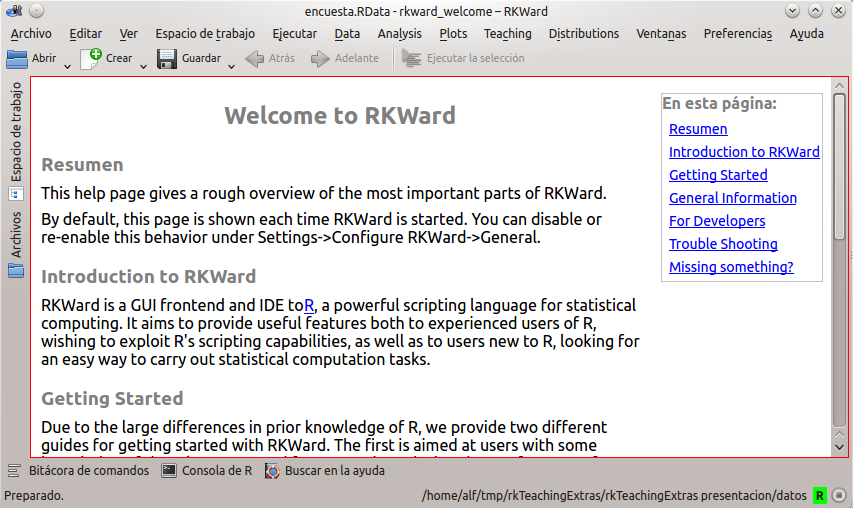
\includegraphics[width=\textwidth]{chapters/introduction/img/rkward}
\end{center}

The main goal of this chapter is to introduce the student to the use of RKWard and rk.Teaching, showing him the basic
operations to enter and manipulate data.

\section{Installation}
The installation of the required software for these practices depends on the operating system.

\subsection{Windows}
For Windows there is an installation bundle that included R, RKWard and rkTeaching. The installation program can be downloaded from \url{https://aprendeconalf.es/en/project/rkteaching/#installation-on-windows}.

\subsection{MacOs}
For MacOs, R must be installed first, after RKWard and finally the package rkTeaching. The steps to do the installation are described at \url{https://aprendeconalf.es/en/project/rkteaching/#installation-on-mac-os}.

\subsection{Linux}
For Linux, R must be installed first, after RKWard and finally the package rkTeaching. The steps to do the installation are described at \url{https://aprendeconalf.es/en/project/rkteaching/#installation-on-linux}.


\section{Solved exercises}
\begin{enumerate}[leftmargin=*]
\item Create a data set with the data in the sample below and save it with name \variable{colesterol.rda}
\begin{center}
\begin{tabular}{|l|c|r|r|r|}
\hline
\multicolumn{1}{|c|}{Name} & \multicolumn{1}{c|}{Gender} & \multicolumn{1}{c|}{Weight} & \multicolumn{1}{c|}{Height} &
\multicolumn{1}{c|}{Cholesterol}\\
\hline
José Luis Martínez Izquierdo  & M &  85 & 179 & 182\\
Rosa Díaz Díaz & F & 65 & 173 & 232\\
Javier García Sánchez  & M & 71 & 181 & 191\\
Carmen López Pinzón & F &  65 & 170 & 200\\
Marisa López Collado & F &  51 & 158 & 148\\
Antonio Ruiz Cruz & M & 66 & 174 & 249\\
\hline
\end{tabular}
\end{center}

\begin{indication}
To create a data set:
\begin{enumerate}
\item Select the menu \menu{File > New > Dataset}.
\item In the dialog displayed enter the name \variable{cholesterol} and click the button \button{OK}.
\item In the data editor window, define a variable in every column giving a name for the variable in the \field{Name}
row, a type (Numeric, Factor, String or Logical) in the \field{Type} row, and in the case of a factor, defining its
levels in the \field{Levels} row.
\item After define the variable, enter the data of every variable in the sample in the corresponding column.
\end{enumerate}
To save the data set:
\begin{enumerate}
\item Select the menu \menu{Workspace > Save Workspace}.
\item In the dialog displayed give the name \variable{cholesterol.rda} to the file, select the folder where to save it
and click the button \button{Save}.
\end{enumerate}
\end{indication}

\item Define a new variable \variable{Age} with the ages of the individuals in the sample, between the variables
\variable{Name} and \variable{Gender}.
\begin{center}
\begin{tabular}{|l|r|}
\hline
\multicolumn{1}{|c|}{Name} & \multicolumn{1}{c|}{Age} \\
\hline
José Luis Martínez Izquierdo & 18 \\
Rosa Díaz Díaz & 32 \\
Javier García Sánchez & 24 \\
Carmen López Pinzón & 35 \\
Marisa López Collado & 46 \\
Antonio Ruiz Cruz & 68 \\
\hline
\end{tabular}
\end{center}

\begin{indication} 
\begin{enumerate}
\item Click the left tab \button{Workspace}.
\item In the workspace window double-click the data set \variable{cholesterol} to edit it.
\item In the data editor window, right-click the column header of the variable \variable{Gender} and select
\menu{Insert new variable left}. 
\item In the new empty column enter the name and type of the variable \variable{Age}, and enter the age of every
individual.
\end{enumerate}
\end{indication}

\item Insert the following data of a new individual:
\begin{quote}
Name: Cristóbal Campos Ruiz.\\
Age: 44 years.\\
Gender: Male.\\
Weight: 70 Kg.\\
Height: 178 cm.\\
Cholesterol: 220 mg/dl.
\end{quote}

\begin{indication}
\begin{enumerate}
\item Insert the data of the new individual in the first empty row.
\end{enumerate}
\end{indication}

\item Create a new variable with the body mass index of every individual using the formula
\[
\text{bmi} = \frac{\text{Weight (in Kg)}}{\text{Height (in m)}^2}
\]

\begin{indication}
\begin{enumerate}
\item Select the menu \menu{Teaching > Data > Compute variable}.
\item In the dialog displayed enter the formula to compute the body mass index in the field \field{Variable
computation}.
\item In the field \field{Save as} click the button \button{Change}.
\item In the dialog displayed select as a parent object the data set \variable{cholesterol} and click
the button \button{OK}.
\item Enter the name \variable{bmi} for the new variable and click the button \button{Submit}.
\end{enumerate}
\end{indication}

\item Recode the body mass index variable into a new categorical variable \variable{Obesity} according to the following
rules:
\begin{center}
\begin{tabular}{lcl}
Less than de $18.5$ & \rightarrow & Low weight\\
From $18.5$ to $24.5$ & \rightarrow & Healthy\\
From $24.5$ to $30$ & \rightarrow & Overweight\\
Greater than $30$  & \rightarrow & Obese
\end{tabular}
\end{center}

\begin{indication}
\begin{enumerate}
\item Select the el menu \menu{Teaching > Data > Variable recoding}.
\item In the dialog displayed insert the variable \variable{bmi} in the field \field{Variable to recode}.
\item Enter the recoding rules below in the field \field{Recoding rules}:
\begin{quote}
\lstinline{lo:18.5 = 1}\\
\lstinline{18.5:24.5 = 2}\\
\lstinline{24.5:30 = 3}\\
\lstinline{30:hi = 4}
\end{quote}
\item In the field \field{Save as} click the button \button{Change}.
\item In the dialog displayed select as a parent object the data set \variable{cholesterol} and click the button
\button{OK}.
\item Enter the name \variable{Obesity} for the new variable and click the button \button{Submit}.
\item In the data edition window, enter the levels for the \variable{Obesity} factor, setting the label ``Low weight''
for the first category, ``Healthy'' for the second one, ``Overweight'' for the third and ``Obese'' for the fourth.
\end{enumerate}
\end{indication}


\item Filter the data set to get a new data set with the data of males. 
\begin{indication}
\begin{enumerate}
\item Select the menu \menu{Teaching > Data > Data filtering}.
\item In the dialog displayed insert the data set \variable{cholesterol} in the field \field{Data set}.
\item Insert the expression \lstinline{gender=="M"} in the field \field{Selection condition}.
\item Enter the name \variable{cholesterol.males} for the new data set and click the button \button{Submit}.
\end{enumerate}
\end{indication}

\end{enumerate}

\section{Proposed exercises}
\begin{enumerate}[leftmargin=*]
\item The data set \variable{neonates} of the package \variable{rk.Teaching}, contains information about a
sample of 320 newborns that meet the normal gestation time in a hospital during one year.
Do the following operations:
\begin{enumerate}
\item Load the data set.
\begin{indication}
\begin{enumerate}
\item Click the \field{Workspace} tab and double-click the \variable{rk.Teaching} package to unfold the data sets that
it contains. 
\item Right-click the data set \variable{nenonates} and select the menu \menu{Copy to .GlobalEnv} to copy the data
set to the working environment.
\end{enumerate}
\end{indication}

\item Compute the variable \variable{APGAR.average} as the mean of the variables \variable{APGAR1} and
\variable{APGAR5}.
\item Recode the variable \variable{weight} into the factor \variable{weight.category} with two categories
corresponding to weights less than and greater than $2.5$ Kg.
\item Recode the variable \variable{APGAR1} into the factor \variable{APGAR.state} with three categories: depressed
(APGAR$\leq 3$), moderately depressed ($3<$APGAR$\leq 6$) and normal (APGAR$>6$).
\item Filter the data set to get a new data set with the neonates of non-smoking mothers with an APGAR score at 1
minute less than or equal to 3.
How many neonates are there?
\end{enumerate}
\end{enumerate}

% Author: Alfredo Sánchez Alberca (asalber@ceu.es)

\chapter{Frequency distributions and charts}\label{cha:freqency-distributions}

\section{Solved exercises}
\begin{enumerate}[leftmargin=*]

\item The number of childre in a sample of 25 is
\begin{center}
1, 2, 4, 2, 2, 2, 3, 2, 1, 1, 0, 2, 2, 0, 2, 2, 1, 2, 2, 3, 1, 2, 2, 1, 2.
\end{center}
Do the following operations:
\begin{enumerate}
\item Create a data frame with the variable \variable{children} and enter the data.

\item Create the frequency table.
\begin{indication}
\begin{enumerate}
\item Select the menu \menu{Teaching > Frequency distribution > Frequency tabulation} .
\item In the dialog displayed, select the variable \variable{children} in the field \field{Variable to tabulate} and
click the button \button{Send}.
\end{enumerate}
\end{indication}

\item Create the absolute frequencies bar chart.
\begin{indication}
\begin{enumerate}
\item Select the menu \menu{Teaching > Gráficos > Diagrama de barras}.
\item In the dialog displayed, select the variable \variable{hijos} in the field \field{Variable} and hacer
clic en el botón \button{Send}.
\end{enumerate}
\end{indication}

\item Para la misma tabla de frecuencias anterior, dibujar también el diagrama de barras de las relative frequencies,
el de absolutas acumuladas and el de relativas acumuladas, además de sus correspondientes polígonos.
\begin{indication}Repetir los pasos del apartado anterior activando, en la solapa de \option{Opciones de las barras},
la opción \option{Frecuencias relativas} si se desea el diagrama de barras de relative frequencies, activando la opción
\option{Frecuencias acumuladas} si se desea el diagrama de barras de frecuencias acumuladas and activando la opción
\option{Polígono} para obtener el polígono asociado.
\end{indication}
\end{enumerate}

\item En un hospital se realizó un estudio sobre el número de personas que ingresaron en urgencias cada día del mes de
noviembre. Los datos observados fueron:
\begin{center}
15, 23, 12, 10, 28, 50, 12, 17, 20, 21, 18, 13, 11, 12, 26 \\
30, 6, 16, 19, 22, 14, 17, 21, 28, 9, 16, 13, 11, 16, 20
\end{center}
Se pide:

\begin{enumerate}
\item  Crear un conjunto de datos con la variable \variable{urgencias} e introducir los datos.

\item  Dibujar el diagrama de cajas. ¿Existe algún dato atípico? En el caso de que exista, eliminarlo and proceder con los
siguientes apartados.
\begin{indication}
\begin{enumerate}
\item Select the menu \menu{Teaching > Gráficos > Diagrama de cajas}.
\item In the dialog displayed, select the variable \variable{urgencias} in the field \field{Variables} y
click the button \button{Send}.
\item En la ventana que aparece con el diagrama de cajas identificar el dato atípico.
\item Ir a la ventana de edición de datos and eliminar la fila del dato atípico haciendo clic con el botón derecho del
ratón en la cabecera de la fila and seleccionando \menu{Borrar esta fila}. 
\end{enumerate}
\end{indication}

\item Construir la tabla de frecuencias agrupando en 5 clases.
\begin{indication}
\begin{enumerate}
\item Select the menu \menu{Teaching > Frequency distribution > Frequency tabulation}.
\item In the dialog displayed select the variable \variable{urgencias}.
\item En la solapa de \option{Clases} activar la casilla \option{Agrupar en intervalos}, marcar la opción \option{Número
de intervalos} e introducir el número deseado de intervalos in the field \field{Intervalos sugeridos} and hacer clic sobre el botón
\button{Send}.
\end{enumerate}
\end{indication}

\item  Dibujar el histograma de absolute frequencies correspondiente a la tabla anterior.
\begin{indication}
\begin{enumerate}
\item Select the menu \menu{Teaching > Gráficos > Histograma}.
\item In the dialog displayed select the variable \variable{urgencias} in the field \field{Variable}.
\item En la solapa de \option{Clases} activar la casilla \option{Agrupar en intervalos}, marcar la opción \option{Número
de intervalos} e introducir el número deseado de intervalos in the field \field{Intervalos sugeridos} and hacer clic sobre el botón
\button{Send}.
\end{enumerate}
\end{indication}

\item Para la misma tabla de frecuencias anterior, dibujar también el histograma de las relative frequencies, el de
absolutas acumuladas and el de relativas acumuladas, además de sus correspondientes polígonos.
\begin{indication}Repetir los pasos del apartado anterior activando, en la solapa de \option{Opciones del histograma},
la opción \option{Frecuencias relativas} si se desea el histograma de relative frequencies, activando la opción
\option{Frecuencias acumuladas} si se desea el histograma de frecuencias acumuladas and activando la opción
\option{Polígono} para obtener el polígono asociado.
\end{indication}
\end{enumerate}

\item Los grupos sanguíneos de una muestra de 30 personas son:
\begin{center}
A, B, B, A, AB, 0, 0, A, B, B, A, A, A, A, AB,\\
A, A, A, B, 0, B, B, B, A, A, A, 0, A, AB, 0. 
\end{center}
Se pide:
\begin{enumerate}
\item Crear un conjunto de datos con la variable \variable{grupo.sanguineo} e introducir los datos.

\item Construir la tabla de frecuencias.
\begin{indication}
\begin{enumerate}
\item Select the menu \menu{Teaching > Frequency distribution > Frequency tabulation} .
\item In the dialog displayed, select the variable \variable{grupo.sanguineo} in the field
\field{Variable to tabulate} and click the button \button{Send}.
\end{enumerate}
\end{indication}

\item Dibujar el diagrama de sectores.
\begin{indication}
\begin{enumerate}
\item Select the menu \menu{Teaching > Gráficos > Diagrama de sectores}.
\item In the dialog displayed, select the variable \variable{grupo.sanguineo} in the field
\field{Variables} and hacer clic sobre el botón \button{Send}.
\end{enumerate}
\end{indication}
\end{enumerate}

\item  En un estudio de población se tomó una muestra de 27 personas, and se les preguntó por su edad and estado civil,
obteniendo los siguientes resultados:
\begin{center}
\begin{tabular}{|l|rrrrrrrrr|}
\hline
Estado civil & \multicolumn{9}{c|}{Edad}\\
\hline
Soltero    & 31 & 45 & 35 & 65 & 21 & 38 & 62 & 22 & 31 \\
Casado     & 62 & 39 & 62 & 59 & 21 & 62 &    &    &    \\
Viudo      & 80 & 68 & 65 & 40 & 78 & 69 & 75 &    &    \\
Divorciado & 31 & 65 & 59 & 49 & 65 &    &    &    &    \\
\hline
\end{tabular}
\end{center}

Se pide:
\begin{enumerate}
\item Crear un conjunto de datos con la variables \variable{estado.civil} and \variable{edad} e introducir los datos.
\item Construir la tabla de frecuencias de la variable \variable{edad} para cada categoría de la
variable \variable{estado.civil}.
\begin{indication}
\begin{enumerate}
\item Select the menu \menu{Teaching > Frequency distribution > Frequency tabulation}.
\item In the dialog displayed, select the variable \variable{edad} in the field \field{Variable a
tabular}, activar la casilla \option{Tabular por grupos}, select the variable \variable{estado.civil} in the field
\field{Variable de agrupación} and click the button \button{Send}.
\end{enumerate}
\end{indication}

\item Dibujar los diagramas de cajas de la edad según el estado civil. ¿Existen datos atípicos? ¿En qué grupo hay mayor
dispersión?
\begin{indication}
\begin{enumerate}
\item Select the menu \menu{Teaching > Gráficos > Diagrama de cajas}.
\item In the dialog displayed, select the variable \variable{edad} in the field \field{Variables},
activar la casilla \option{Dibujar por grupos}, select the variable \variable{estado.civil} in the field
\field{Variable de agrupación} and click the button \button{Send}.
\end{enumerate}
\end{indication}
\end{enumerate}

\end{enumerate}


\section{Ejercicios propuestos}
\begin{enumerate}[leftmargin=*]

\item  El número de lesiones padecidas durante una temporada por cada jugador de un equipo de fútbol fue el siguiente:
\begin{center}
0, 1, 2, 1, 3, 0, 1, 0, 1, 2, 0, 1, 1, 1, 2, 0, 1, 3, 2, 1, 2, 1, 0, 1
\end{center}

Se pide:
\begin{enumerate}
\item Construir la tabla de frecuencias.
\item Dibujar el diagrama de barras de las relative frequencies and de relative frequencies acumuladas.
\item Dibujar el diagrama de sectores.
\end{enumerate}

\item Para realizar un estudio sobre la estatura de los estudiantes universitarios, seleccionamos, mediante un proceso
de muestreo aleatorio, una muestra de 30 estudiantes, obteniendo los siguientes resultados (medidos en centímetros):
\begin{center}
179, 173, 181, 170, 158, 174, 172, 166, 194, 185,\\
162, 187, 198, 177, 178, 165, 154, 188, 166, 171,\\
175, 182, 167, 169, 172, 186, 172, 176, 168, 187.
\end{center}

Se pide:
\begin{enumerate}
\item Dibujar el histograma de las absolute frequencies agrupando desde 150 a 200 en clases de amplitud 10.
\item Dibujar el diagrama de cajas. ¿Existe algún dato atípico?.
\end{enumerate}

\item El conjunto de datos \variable{neonatos} del paquete \variable{rk.Teaching}, contiene información sobre una
muestra de 320 recién nacidos en un hospital durante un año que cumplieron el tiempo normal de gestación. 
Se pide:
\begin{enumerate}
\item Construir la tabla de frecuencias de la puntuación Apgar al minuto de nacer. 
Si se considera que una puntuación Apgar de 3 o menos indica que el neonato está deprimido, ¿qué porcentaje de niños está deprimido en la muestra?
\item Comparar las distribuciones de frecuencias de las puntuaciones Apgar al minuto de nacer según si la madre es mayor
o menor de 20 años.
¿En qué grupo hay más neonatos deprimidos?
\item Construir la tabla de frecuencias para el peso de los neonatos, agrupando en clases de amplitud $0.5$ desde el
$2$ hasta el $4.5$. ¿En qué intervalo de peso hay más niños?
\item Comparar la distribución de relative frequencies del peso de los neonatos según si la madre fuma o no. Si se
considera como peso bajo un peso menor de $2.5$ kg, ¿En qué grupo hay un mayor porcentaje de niños con peso bajo?
\item Si en los recién nacidos se considera como peso bajo un peso menor de $2.5$ kg, calcular la prevalencia del bajo
peso de recién nacidos en el grupo de madres fumadoras and en el de no fumadoras. 
\item Calcular el riesgo relativo de que un recién nacido tenga bajo peso cuando la madre fuma, frente a cuando la madre
no fuma. 
\item Construir el diagrama de barras de la puntuación Apgar al minuto. ¿Qué puntuación Apgar es la más frecuente? 
\item Construir el diagrama de relative frequencies acumuladas de la puntuación Apgar al minuto. ¿Por debajo de que puntuación estarán la mitad de los niños?
\item Comparar mediante diagramas de barras de relative frequencies las distribuciones de las puntuaciones Apgar al
minuto según si la madre ha fumado o no durante el embarazo. ¿Qué se puede concluir?
\item Construir el histograma de pesos, agrupando en clases de amplitud $0.5$ desde el $2$ hasta el $4.5$. ¿En qué
intervalo de peso hay más niños?
\item Comparar la distribución de relative frequencies del peso de los neonatos según si la madre fuma o no. ¿En qué
grupo se aprecia menor peso de los niños de la muestra?
\item Comparar la distribución de relative frequencies del peso de los neonatos según si la madre fumaba o no antes del
embarazo. ¿Qué se puede concluir?
\item Construir el diagrama de caja and bigotes del peso. ¿Entre qué valores se considera que el peso de un neonato es
normal? ¿Existen datos atípicos?
\item Comparar el diagrama de cajas and bigotes del peso, según si la madre fumó o no durante el embarazo and si era mayor o
no de 20 años. ¿En qué grupo el peso tiene más dispersión central? ¿En qué grupo pesan menos los niños de la
muestra?
\item Comparar el diagrama de cajas de la puntuación Apgar al minuto and a los cinco minutos. ¿En qué variable hay más
dispersión central?
\end{enumerate}  

\end{enumerate}

% Author: Alfredo Sánchez Alberca (asalber@ceu.es)

\chapter{Sampling statistics}\label{cha:statistics}

\section{Solved exercises}
\begin{enumerate}[leftmargin=*]
\item The number of children in a sample of 25 families is
\begin{center}
1, 2, 4, 2, 2, 2, 3, 2, 1, 1, 0, 2, 2, 0, 2, 2, 1, 2, 2, 3, 1, 2, 2, 1, 2.
\end{center}
Do the following operations:
\begin{enumerate}
\item Create a data set with the variable \variable{children} and enter the data.
\item Compute the arithmetic mean, variance and standard deviation of the number of children.
Interpret the statistics.
\begin{indication}
\begin{enumerate}
\item Select the menu \menu{Teaching >  Descriptive statistics >  Statistics}.
\item In the dialog displayed insert the variable \variable{children} in the field \field{Variable}.
\item In the \mtab{Basic statistics} tab check the boxes of \option{Arithmetic mean}, \option{Variance} and
\option{Standard deviation}, and click the button \button{Submit}.
\end{enumerate}
\end{indication}

\item Compute the quartiles, the range, the interquartile range, the third decile and the 68th percentile. 
\begin{indication}
\begin{enumerate}
\item Select the menu \menu{Teaching >  Descriptive statistics >  Statistics}.
\item In the dialog displayed insert the variable \variable{children} in the field \field{Variable}.
\item In the \mtab{Basic statistics} tab check the boxes of \option{Quartiles}, \option{Range}, \option{Interquartile
range}, enter the values $0.3$ and $0.68$ in the field $\field{Percentiles}$, and click the button \button{Submit}.
\end{enumerate}
\end{indication}
\end{enumerate}

\item The number of people treated in the emergency service of a hospital every day of November was
\begin{center}
15 \quad 23 \quad 12 \quad 10 \quad 28 \quad 7 \quad 12 \quad 17 \quad 20 \quad 21 \quad 18 \quad 13 \quad 11 \quad 12 \quad 26 \\
30 \quad 6 \quad 16 \quad 19 \quad 22 \quad 14 \quad 17 \quad 21 \quad 28 \quad 9 \quad 16 \quad 13 \quad 11 \quad 16 \quad 20
\end{center}
Do the following operations: 
\begin{enumerate}
\item Create a data set with the variable \variable{emergencies} and enter the data.

\item Compute the arithmetic mean, variance, standard deviation and coefficient of variation of the number of
emergencies.
Interpret the statistics. 
\begin{indication}
\begin{enumerate}
\item Select the menu \menu{Teaching >  Descriptive statistics >  Statistics}.
\item In the dialog displayed insert the variable \variable{emergencies} in the field \field{Variable}.
\item In the \mtab{Basic statistics} tab check the boxes of \option{Arithmetic mean}, \option{Variance}, 
\option{Standard deviation} and \option{Coefficient of variation}, and click the button \button{Submit}.
\end{enumerate}
\end{indication}

\item Compute the coefficients of skewness and kurtosis and interpret the statistics.
\begin{indication}
\begin{enumerate}
\item Select the menu \menu{Teaching >  Descriptive statistics >  Statistics}.
\item In the dialog displayed insert the variable \variable{emergencies} in the field \field{Variable}.
\item In the \mtab{Basic statistics} tab check the boxes of \option{Coefficient of skewness} and \option{Coefficient
of kurtosis} and click the button \button{Submit}.
\end{enumerate}
\end{indication}
\end{enumerate}


\item In a group of 20 students the grades in Mathematics were
\begin{center}
SS, AP, SS, AP, AP, NT, NT, AP, SB, SS \\
SB, SS, AP, AP, NT, AP, SS, NT, SS, NT
\end{center}

Do the following operations:
\begin{enumerate}
\item  Create a data set \variable{course} with the variable \variable{grades} and enter the data.

\item  Recode the grades into scores assigning $2.5$ to SS, $6$ to AP, $8$ to NT and $9.5$ to SB.
\begin{indication}
\begin{enumerate}
\item Select the menu \menu{Teaching > Data > Variable recoding}.
\item In the dialog displayed insert the \variable{grades} in the field \field{Variable to recode}.
\item Enter the following recoding rules in the field \field{Recoding rules}:
\begin{quote}
\lstinline{"SS" = 2.5}\\
\lstinline{"AP" = 6}\\
\lstinline{"NT" = 8}\\
\lstinline{"SB" = 9.5}
\end{quote}
\item In the \field{Save new variable} click the button \button{Change}.
\item In the dialog displayed select as parent object the data set \variable{course} and click
the button \button{Accept}.
\item Enter the name \variable{score} for the new variable, uncheck the box \option{Convert in a factor} and click the
button \button{Submit}.
\end{enumerate}
\end{indication}

\item Compute the median and the interquartile range.
\begin{indication}
\begin{enumerate}
\item Select the menu \menu{Teaching >  Descriptive statistics >  Statistics}.
\item In the dialog displayed select the variable \variable{score} in the field \field{Variable}.
\item In the \mtab{Basic statistics} tab check the boxes of \option{Median} and \option{Interquartile range} and click the button \button{Submit}.
\end{enumerate}
\end{indication}
\end{enumerate}

\item The heights of a sample of 30 students are:
\begin{center}
\begin{tabular}{ll}
Females: & 173, 158, 174, 166, 162, 177, 165, 154, 166, 182, 169, 172, 170, 168. \\
Males: & 179, 181, 172, 194, 185, 187, 198, 178, 188, 171, 175, 167, 186, 172, 176, 187.
\end{tabular}
\end{center}

Do the following operations:
\begin{enumerate}
\item Create a data set with the variables \variable{height} and \variable{gender} and enter the data.

\item Compute the arithmetic mean, median, variance, standard deviation and quartiles according to the gender.
Interpret the statistics.
\begin{indication}
\begin{enumerate}
\item Select the menu \menu{Teaching >  Descriptive statistics >  Statistics}.
\item In the dialog displayed insert the variable \variable{height} in the field \field{Variable},
check the box \option{Statistics by groups} and insert the variable \variable{gender} in the field \field{Grouping
variable(s)}.
\item In the \mtab{Basic statistics} tab check the boxes of \option{Arithmetic mean}, \option{Median},
\option{Variance}, \option{Standard deviation} and \option{Quartiles}, and click the button \button{Submit}.
\end{enumerate}
\end{indication}
\end{enumerate}

\end{enumerate}


\section{Proposed exercises}
\begin{enumerate}[leftmargin=*]
\item The number of injuries suffered by the members of a soccer team in a league were
\begin{center}
0, 1, 2, 1, 3, 0, 1, 0, 1, 2, 0, 1, 1, 1, 2, 0, 1, 3, 2, 1, 2, 1, 0, 1
\end{center}

Do the following operations:
\begin{enumerate}
\item Compute la arithmetic mean, median, variance and standard deviation of the number of injuries and interpret them.
\item Compute the coefficients of skewness and kurtosis.
\item Compute the fourth and the eighth deciles and interpret them.
\end{enumerate}

\item We want to compare the reliability of two blood pressure monitors, an arm monitor and a wrist monitor. 
For that purpose we have performed 8 repeated measures of the blood pressure of the same person with both moniors.
The measurements (in mmHg) were:
\begin{center}
\begin{tabular}{rl}
Arm monitor: & 111, 109, 112, 111, 113, 113, 114, 111\\
Wrist monitor: & 115, 113, 117, 116, 112, 112, 117, 112
\end{tabular}
\end{center}
Which monitor is more reliable?

\item The age and the marital status of a sample of 28 persons are:
\begin{center}
\begin{tabular}{|l|rrrrrrrrr|}
\hline
Marital status & \multicolumn{9}{c|}{Age}\\
\hline
Single    & 31 & 45 & 35 & 65 & 21 & 38 & 62 & 22 & 31 \\
Married     & 72 & 39 & 62 & 59 & 25 & 44 & 54 &    &    \\
Widow(er)      & 80 & 68 & 65 & 40 & 78 & 69 & 75 &    &    \\
Divorced & 31 & 65 & 59 & 58 & 50 &    &    &    &    \\
\hline
\end{tabular}
\end{center}

Do the following operations:
\begin{enumerate}
\item Compute the arithmetic mean and the standard deviation of the age according to the marital status and interpret
them.
\item What group has the most representative mean?
\end{enumerate}

\item A study wants to determine if there are relations between the blood pressure and the tobacco and drink. 
The values observed in a sample of 25 persons were:
\begin{center}
\begin{tabular}{lccccccccccccc}
\hline
Smokes  & yes & no & yes & yes & yes & no & no & yes & no & yes & no & yes & no \\
Drinks & no & no & yes & yes & no & no & yes & yes & no & yes & no & yes & yes \\
Blood pressure & 80 & 92 & 75 & 56 & 89 & 93 & 101 & 67 & 89 & 63 & 98 & 58 & 91 \\
\hline
\\
\hline
Smokes  & yes & no & no & yes & no & no & no & yes & no & yes & no & yes \\
Drink & yes & no & yes & yes & no & no & yes & yes & yes & no & yes & no \\
Blood pressure & 71 & 52 & 98 & 104 & 57 & 89 & 70 & 93 & 69 & 82 & 70 & 49 \\
\hline
\end{tabular}
\end{center}

\begin{enumerate}
\item Compute the arithmetic mean, the standard deviation and the coefficients of skewness and kurtosis of the blood
pressure for smokers and non-smokers, and interpret them.
\item Compute the same statistics for drinkers and non-drinkers. Interpret the statistics.
\item Compute the same statistics for smokers and drinkers, smokers and non-drinkers, non-smokers and drinkers, and
non-smoker and non-drinkers. Interpret the statistics
\end{enumerate}


% \item El conjunto de datos \variable{neonatos} del paquete \variable{rk.Teaching}, contiene información sobre una
% muestra de 320 recién nacidos en un hospital durante un año que cumplieron el tiempo normal de gestación. 
% Do the following operations:
% \begin{enumerate}
% \item Compute la media and la median muestral del peso de los nacidos e interpretarlos. 
% \item Compute el peso medio de los recién nacidos de la muestra según si la madre ha fumado o no durante el embarazo.
% Compute también el peso medio de los recién nacidos de madres que no han fumado durante el embarazo, según si la madre
% fumaba o no antes del embarazo. ¿Qué conclusiones se pueden sacar?
% \item ¿Cuál es la puntuación Apgar al minuto de nacer más frecuente?
% \item Compute la media de la diferencia entre las puntuaciones Apgar a los 5 minutos and al minuto de nacer. ¿Cómo
% evolucionan los recién nacidos?
% \item Compute los quartiles muestrales del peso de los recién nacidos e interpretarlos.
% \item Comparar los quartiles muestrales del peso de los recién nacidos según el gender. 
% \item ¿Por encima de qué peso estarán el 10\% de los niños con mayor peso?
% \item Si se considera que un niño es atípico por bajo peso si se encuentra entre el 5\% de los pesos más bajos, ¿por
% debajo de qué peso tiene que estar?
% \item Compute el recorrido and el range intercuartílico muestrales del peso de los recién nacidos e interpretarlos.
% \item Compute la variance and la standard deviation del peso de los recién nacidos e interpretarlos.
% \item ¿En qué grupo hay más variabilidad del peso de los recién nacidos, en las madres fumadoras o en las madres no
% fumadoras durante el embarazo? ¿En qué grupo será más representativo el peso medio?
% \item ¿Qué variable presenta más variabilidad relativa, el peso de los recién nacidos o el Apgar al minuto de nacer?
% \item Compute el coefficient of skewness and de apuntamiento muestrales del peso de los recién nacidos e interpretarlos.
% \item ¿Qué distribución es más asimétrica, la de los pesos de recién nacidos en madres mayores de 20 años o en madres
% menores de 20 años?
% \item ¿Qué distribución es más apuntada, la del peso de los recién nacidos en hombres o en mujeres?
% \item De acuerdo a la forma de la distribución, ¿puede considerarse la puntuación Apgar al minuto de nacer como una
% variable normal? ¿Y el número de cigarros fumados al día durante el embarazo?
% \end{enumerate}
\end{enumerate}

% Author: Alfredo Sánchez Alberca (asalber@ceu.es)

\chapter{Linear regression}\label{cha:linear-regression}

\section{Solved exercises}
\begin{enumerate}[leftmargin=*]
\item The values of two variables $X$ and $Y$ measured in a sample of 10 individuals are:
\[
\begin{array}{lrrrrrrrrrr}
\hline
X & 0 & 1 & 2 & 3 & 4 & 5 & 6 & 7 & 8 & 9 \\
Y & 2 & 5 & 8 & 11 & 14 & 17 & 20 & 23 & 26 & 29\\
\hline
\end{array}
\]

Do the following operations:

\begin{enumerate}
\item Create a data set with the variables \variable{X} and \variable{Y} amd enter the data.
\item Construct the scatter plot of \variable{X} and \variable{Y}.
\begin{indication}
\begin{enumerate}
\item Select the menu \menu{Teaching > Charts > Scatter plot}.
\item In the dialog displayed, select the variable \variable{Y} in the field \field{Variable Y}, and the variable
\variable{X} in the field \field{Variable X}, and click the button \button{Submit}.
\end{enumerate}
\end{indication}

According to the point cloud, what type of regression model explains better the relation between \variable{X} and
\variable{Y}?

\item Compute the regression line of $Y$ on $X$.
\begin{indication}
\begin{enumerate}
\item Select the menu \menu{Teaching > Regression > Linear regression}.
\item In the dialog displayed, insert the variable \variable{Y} in the field \field{Dependent variable} and the variable
\variable{X} in the field \field{Independent variable}, and click the button \button{Submit}.
\end{enumerate}
\end{indication}

\item Plot the regression line on the scatter plot.
\begin{indication}
\begin{enumerate}
\item Select the menu \menu{Teaching > Charts > Scatter plot}.
\item In the dialog displayed, insert the variable \variable{Y} in the field \field{Variable Y} and the
variable \variable{X} in the field \field{Variable X}.
\item In the \menu{Fitted line} tab, check the box \option{Linear} and click the button
\button{Submit}.
\end{enumerate}
\end{indication}

\item Compute la regression line of $X$ on $Y$ and plot it on the scatter plot.
\begin{indication}
Repeat the steps of the previous part but inserting the variable \variable{X} in the field \field{Dependent variable}
and the variable \variable{Y} in the field \field{Independent variable}. 
\end{indication}

\item How are the residuals?
Comment the results.
\end{enumerate}


\item  En una licenciatura se quiere estudiar la relación entre el número medio de horas de estudio diarias and el número
de asignaturas suspensas. Para ello se obtuvo la siguiente muestra:
\[
\begin{array}{cccccccc}
\text{Horas} & \text{Suspensos} &  & \text{Horas} & \text{Suspensos} & & \text{Horas} & \text{Suspensos}  \\
\cline{1-2}\cline{4-5}\cline{7-8}
3.5 & 1 & & 2.2 & 2 & & 1.3 & 4 \\
0.6 & 5 & & 3.3 & 0 & & 3.1 & 0 \\
2.8 & 1 & & 1.7 & 3 & & 2.3 & 2 \\
2.5 & 3 & & 1.1 & 3 & & 3.2 & 2 \\
2.6 & 1 & & 2.0 & 3 & & 0.9 & 4 \\
3.9 & 0 & & 3.5 & 0 & & 1.7 & 2 \\
1.5 & 3 & & 2.1 & 2 & & 0.2 & 5 \\
0.7 & 3 & & 1.8 & 2 & & 2.9 & 1 \\
3.6 & 1 & & 1.1 & 4 & & 1.0 & 3 \\
3.7 & 1 & & 0.7 & 4 & & 2.3 & 2 \\
\end{array}
\]

Do the following operations:
\begin{enumerate}
\item  Create a data set con las variables \variable{horas.estudio} and \variable{suspensos} e introducir estos
datos.

\item Construir la frequency table bidimensional de las variables \variable{horas.estudio} and \variable{suspensos}. 
\begin{indication}
\begin{enumerate}
\item Select the menu \menu{Teaching > Frequency distribution > Tabla de frecuencias bidimensional}.
\item In the dialog displayed, select the variable \variable{horas.estudio} in the field \field{Variable
a tabular en filas}, la variable \variable{suspensos} in the field \field{Variable a tabular en columnas}, and hacer clic
sobre el botón \button{Submit}. 
\end{enumerate}
\end{indication}

\item  Compute la regression line of \variable{suspensos} sobre \variable{horas.estudio} and dibujarla.
\begin{indication}
Para calcular la recta de regresión:
\begin{enumerate}
\item Select the menu \menu{Teaching > Regression > Linear regression}.
\item In the dialog displayed, select the variable \variable{suspensos} in the field \field{Variable
dependiente} and la variable \variable{horas.estudio} in the field \field{Independent variable}, seleccionar
\option{Guardar el modelo}, introducir un nombre para el modelo and click the button \button{Submit}.
\end{enumerate}
Para dibujar la recta de regresión:
\begin{enumerate}
\item Select the menu \menu{Teaching > Charts > Scatter plot}.
\item In the dialog displayed, select the variable \variable{suspensos} in the field \field{Variable Y} y
la variable \variable{horas.estudio} in the field \field{Variable X}.
\item En la solapa \menu{Fitted line}, seleccionar \option{Lineal} and click the button
\button{Submit}.
\end{enumerate}
\end{indication}

\item Indicar el coeficiente de regresión de \variable{suspensos} sobre \variable{horas.estudio}. 
¿Cómo lo interpretarías?
\begin{indication}
El coeficiente de regresión es la pendiente de la recta de regresión.
\end{indication}

\item La relación lineal entre estas dos variables, ¿es mejor o peor que la del ejercicio anterior? 
Comentar los resultados a partir las gráficas de las rectas de regresión and sus residuos.

\item Compute los coeficientes de correlación and de determinación lineal. 
¿Es un buen modelo la recta de regresión?
¿Qué porcentaje de la variabilidad del número de suspensos está explicada por el modelo?
\begin{indication}
El coeficiente de determinación aparece en la ventana de resultados como \result{R$^2$}, and el
coeficiente de correlación es su raíz cuadrada.
\end{indication}

\item Utilizar la recta de regresión para predecir el número de suspensos correspondiente a 3 horas de estudio diarias.
¿Es fiable esta predicción? 
\begin{indication}
\begin{enumerate}
\item Select the menu \menu{Teaching > Regression > Predicciones}.
\item In the dialog displayed seleccionar como modelo de regresión la recta calculada en el segundo
apartado, introducir los valores para los que se desea la predicción in the field \field{Predicciones para} and hacer clic
sobre el botón \button{Submit}.
\end{enumerate}
\end{indication}

\item Según el modelo lineal, ¿cuántas horas diarias tendrá que estudiar como mínimo un alumno si quiere aprobarlo
todo?
\begin{indication}
Seguir los mismos pasos de los apartados anteriores, pero escogiendo como variable dependiente \variable{horas.estudio},
y como independiente \variable{suspensos}, and haciendo la predicción para 0 suspensos.
\end{indication}
\end{enumerate}


\item Después de tomar un litro de vino se ha medido la concentración de alcohol en la sangre en distintos instantes,
obteniendo:
\[
\begin{array}{lrrrrrrr}
\hline 
\mbox{Tiempo después (minutos)} & 30 & 60 & 90 & 120 & 150 & 180 & 210\\ 
\mbox{Concentración (gramos/litro)} & 1.6 & 1.7 & 1.5 & 1.1 & 0.7 & 0.2 & 2.1\\
\hline
\end{array}
\]

Do the following operations:
\begin{enumerate}
\item Crear las variables \variable{tiempo} and \variable{alcohol} e introducir estos datos.
\item Compute el coeficiente de correlación lineal entre el alcohol and el tiempo e interpretarlo. ¿Es bueno el modelo
lineal? 
\begin{indication}
\begin{enumerate}
\item Select the menu \menu{Teaching > Regression > Linear regression}.
\item In the dialog displayed, select the variable \variable{alcohol} in the field \field{Variable
dependiente} and la variable \variable{tiempo} in the field \field{Independent variable}, and click the button
\button{Submit}.
\end{enumerate}
\end{indication}

\item Dibujar la regression line ofl alcohol sobre el tiempo. 
¿Existe algún individuo con un residuo demasiado grande? 
Si es así, eliminar dicho individuo de la muestra and volver a calcular el coeficiente de correlación. 
¿Ha mejorado el modelo?
\begin{indication}
\begin{enumerate}
\item Select the menu \menu{Teaching > Charts > Scatter plot}.
\item In the dialog displayed, select the variable \variable{alcohol} in the field \field{Variable Y} y
la variable \variable{tiempo} in the field \field{Variable X}.
\item En la solapa \menu{Fitted line}, seleccionar \option{Lineal} and click the button \button{Submit}.
\end{enumerate}
Se observa que hay un residuo atípico para el punto que corresponde al los 210 minutos. 
Para eliminarlo:
En la ventana de edición del conjunto de datos hacer clic con el botón derecho del ratón sobre la fila correspondiente
al dato con el residuo atípico and seleccionar \option{Borrar esta fila}.
\end{indication}

\item Si la concentración máxima de alcohol en la sangre que permite la ley para poder conducir es $0.3$ g/l, ¿cuánto
tiempo habrá que esperar después de tomarse un litro de vino para poder conducir sin infringir la ley? 
¿Es fiable esta predicción?
\begin{indication}
Para construir la recta de regresión:
\begin{enumerate}
\item Select the menu \menu{Teaching > Regression > Linear regression}.
\item In the dialog displayed, select the variable \variable{tiempo} in the field \field{Variable
dependiente} and la variable \variable{alcohol} in the field \field{Independent variable}.
\item Seleccionar \option{Guardar el modelo}, introducir un nombre para el modelo and click the button \button{Submit}.
\end{enumerate}
Para hacer la predicción:
\begin{enumerate}
\item Select the menu \menu{Teaching > Regression > Predicciones}.
\item In the dialog displayed seleccionar como modelo de regresión la recta calculada e introducir los
valores para los que se desea la predicción in the field \field{Predicciones para} and click the button
\button{Submit}.
\end{enumerate}
\end{indication}
\end{enumerate}


\item El conjunto de datos \variable{edad.estatura} del paquete \variable{rk.Teaching} contine la edad and la estatura
de 30 personas. 
Do the following operations:
\begin{enumerate}
\item Cargar datos del conjunto de datos \variable{edad.estatura} desde el paquete \variable{rk.Teaching}.

\item Compute la regression line of la estatura sobre la edad. ¿Es un buen modelo la recta de regresión?
\begin{indication}
\begin{enumerate}
\item Select the menu \menu{Teaching > Regression > Linear regression}.
\item In the dialog displayed, select the variable \variable{estatura} in the field \field{Variable
dependiente} and la variable \variable{edad} in the field \field{Independent variable}, and click the button
\button{Submit}.
\end{enumerate}
\end{indication}

\item Dibujar el diagrama de dispersión de la estatura sobre la edad. 
¿Alrededor de qué edad se observa un cambio en la tendencia? 
\begin{indication}
\begin{enumerate}
\item Select the menu \menu{Teaching > Charts > Scatter plot}.
\item In the dialog displayed, select the variable \variable{estatura} in the field \field{Variable Y},
la variable \variable{edad} in the field \field{Variable X}, and click the button \button{Submit}.
\end{enumerate}
\end{indication}

\item Recodificar la variable edad en dos grupos para mayores and menores de 20 años.
\begin{indication}
\begin{enumerate}
\item Select the menu \menu{Teaching >  Datos > Recodificar variable}.
\item In the dialog displayed seleccionar in the field \vampo{Variable a recodificar} la variable
\variable{edad}.
\item En el campo \field{Reglas de recodificación} introducir
\begin{quote}
\lstinline{lo:20 = "menores"}\\
\lstinline{20:hi = "mayores"}
\end{quote}
\item En el cuadro \field{Guardar nueva variable} click the button \button{Cambiar}.
\item In the dialog displayed seleccionar como objeto padre la el conjunto de datos \variable{edad\_estatura} and click the button \button{Aceptar}.
\item Introducir el nombre de la nueva variable \variable{grupo.edad} and click the button \button{Submit}.
\end{enumerate}
\end{indication}

\item Compute la regression line of la estatura sobre la edad para cada grupo de edad. 
¿En qué grupo explica mejor la recta de regresión la relación entre la estatura and la edad? 
Justificar la respuesta.
\begin{indication}
\begin{enumerate}
\item Select the menu \menu{Teaching > Regression > Linear regression}.
\item In the dialog displayed, select the variable \variable{estatura} in the field \field{Variable
dependiente} and la variable \variable{edad} como \field{Independent variable}.
\item Seleccionar la opición \option{Ajuste por grupos}, introducir la variable \variable{grupo.edad} in the field
\field{Grouping variable(s)}, and hacer clic en el \button{Submit}.
\end{enumerate}
\end{indication}

\item Dibujar las rectas de regresión anteriores.
\begin{indication}
\begin{enumerate}
\item Select the menu \menu{Teaching > Charts > Scatter plot}.
\item In the dialog displayed, select the variable \variable{estatura} in the field \field{Variable Y} y
la variable \variable{edad} in the field \field{Variable X}.
\item Seleccionar la opción \option{Plot by groups} e introducir la variable \variable{grupo.edad} in the field
\field{Grouping variable(s)}.
\item En la solapa \menu{Fitted line}, seleccionar \option{Lineal} and click the button
\button{Submit}.
\end{enumerate}
\end{indication}

\item ¿Qué estatura se espera que tenga una persona de 14 años? ¿Y una de 38?
\begin{indication}
Para predecir la estatura de la persona de 14 años:
\begin{enumerate}
\item Select the menu \menu{Teaching > Regression > Predicciones}.
\item In the dialog displayed seleccionar como modelo de regresión la recta calculada para los menores e
introducir 14 in the field \field{Predicciones para} and click the button
\button{Submit}.
\end{enumerate}
para predecir la estatura de la persona de 38 años, repetir lo mismo pero seleccionando la recta de regresión para los
mayores e introducidento 38 in the field \field{Predicciones para}.
\end{indication}
\end{enumerate}

\opt{largo}{
\item La siguiente tabla recoge la información de las calificaciones obtenidas por un grupo de alumnos en dos
asignaturas $X$ e $Y$.
\begin{center}
\begin{tabular}{lcccccccccccc}
Alumno & 1 & 2 & 3 & 4 & 5 & 6 & 7 & 8 & 9 & 10 & 11 & 12\\
\hline
$X$ & NT & AP & SS & SS & AP & AP & SS & NT & SB & SS & AP & AP\\
$Y$ & SB & SS & AP & SS & AP & NT & SS & NT & NT & AP & AP & NT
\end{tabular}
\end{center}
Do the following operations:
\begin{enumerate}
\item Create a data set con las variables \varaible{X} e \variable{Y} and enter the data.

\item ¿Existe relación entre las calificaciones de $X$ e $Y$? Justificar la respuesta.
\begin{indication}
\begin{enumerate}
\item Select the menu \menu{Teaching > Regression > Correlación}.
\item In the dialog displayed select the variables \variable{X} e \variable{Y} in the field
\field{Variables}.
\item En la solapa \menu{Opciones de correlación} seleccionar el método de \option{Ro de Spearman} and hacer clic sobre
el botón \button{Submit}.
\end{enumerate}
\end{indication}
\end{enumerate}
}
\end{enumerate}


\section{Proposed exercises}
\begin{enumerate}[leftmargin=*]
\item  Se determina la pérdida de actividad que experimenta un medicamento desde el momento de su fabricación a lo
largo del tiempo, obteniéndose el siguiente resultado:
\begin{center}
\begin{tabular}{|l|c|c|c|c|c|}
\hline 
Tiempo (en años) & 1 & 2 & 3 & 4 & 5 \\ 
\hline 
Actividad restante (\%) & 96 & 84 & 70 & 58 & 52 \\ 
\hline
\end{tabular}
\end{center}
Se desea calcular:
\begin{enumerate}
\item  La relación fundamental (recta de regresión) entre actividad restante and tiempo transcurrido.
\item ¿En qué porcentaje disminuye la actividad cada año que pasa?
\item ¿Cuándo tiempo debe pasar para que el fármaco tenga una actividad del 80\%? ¿Cuándo será nula la actividad?
¿Son igualmente fiables estas predicciones?
\end{enumerate}

\item Al realizar un estudio sobre la dosificación de un cierto medicamento, se trataron 6 pacientes con dosis diarias
de 2 mg, 7 pacientes con 3 mg and otros 7 pacientes con 4 mg. De los pacientes tratados con 2 mg, 2 curaron al cabo de 5
días, and 4 al cabo de 6 días. De los pacientes tratados con 3 mg diarios, 2 curaron al cabo de 3 días, 4 al cabo de 5
días and 1 al cabo de 6 días. Y de los pacientes tratados con 4 mg diarios, 5 curaron al cabo de 3 días and 2 al cabo de 4
días. Do the following operations: 
\begin{enumerate}
\item Compute la regression line ofl tiempo de curación con respecto a la dosis suministrada.
\item Compute el coeficiente de regresión del tiempo de curación con respecto a la dosis e interpretarlo.
\item Compute el coeficiente de correlación lineal e interpretarlo.
\item Determinar el tiempo esperado de curación para una dosis de 5 mg diarios. ¿Es fiable esta predicción?
\item ¿Qué dosis debe aplicarse si queremos que el paciente tarde 4 días en curarse? ¿Es fiable la predicción?
\end{enumerate}

\item El fichero \variable{estaturas.pesos.alumnos} del paquete \variable{rk.Teaching}, contiene la estatura, el peso y
el sexo de una muestra de alumnos universitarios.
Do the following operations:
\begin{enumerate}
\item Cargar el conjunto de datos \variable{estaturas.pesos.alumnos} desde el paquete \variable{rk.Teaching}.
\item Compute la regression line ofl peso sobre la estatura and dibujarla.
\item Compute las rectas de regresión del peso sobre la estatura para cada sexo and dibujarlas.
\item Compute los coeficientes de determinación de ambas rectas. ¿Qué recta es mejor modelo? Justificar la respuesta.
\item ¿Qué peso tendrá un hombre que mida 170 cm? ¿Y una mujer de la misma estatura?
\end{enumerate}

\item El conjunto de datos \variable{neonatos} del paquete \variable{rk.Teaching}, contiene información sobre una
muestra de 320 recién nacidos en un hospital durante un año que cumplieron el tiempo normal de gestación. 
Do the following operations:
\begin{enumerate}
\item Construir la frequency table bidimensional del Agpar al minuto de nacer frente a si la madre ha fumado o no
durante el embarazo. ¿Qué conclusiones se pueden sacar?
\item Construir la frequency table bidimensional del peso de los recién nacidos frente a la edad de la madre. ¿Qué
conclusiones se pueden sacar?
\item Construir la regression line ofl peso de los recién nacidos sobre el número de cigarros fumados al día por las
madres. ¿Existe una relación lineal fuerte entre el peso and el número de cigarros?
\item Dibujar la recta de regresión calculada en el apartado anterior. ¿Por qué la recta no se ajusta bien a la nube de
puntos?
\item Compute and dibujar la regression line ofl peso de los recién nacidos sobre el número de cigarros fumados al día
por las madres en el grupo de las madres que si fumaron durante el embarazo. ¿Es este modelo mejor o pero que la recta
de los apartados anteriores? 

Según este modelo, ¿cuánto disminuirá el peso del recién nacido por cada cigarro más diario
que fume la madre? 
\item Según el modelo anterior, ¿qué peso tendrá un recién nacido de una madre que ha fumado 5 cigarros diarios durante
el embarazo? ¿Y si la madre ha fumado 30 cigarros diarios durante el embarazo? ¿Son fiables estas predicciones?
\item ¿Existe la misma relación lineal entre el peso de los recién nacidos and el número de cigarros fumados al día por
las madres que fumaron durante el embarazo en el grupo de las madres menores de 20 and en el grupo de las madres mayores de
20? ¿Qué se puede concluir?
\end{enumerate}
\end{enumerate}
% Author: Alfredo Sánchez Alberca (asalber@ceu.es)

\chapter{Non-linear regression}\label{cha:non-linear-regression}

\section{Solved exercises}
\begin{enumerate}[leftmargin=*]
\item The number of bacteria in a culture evolves with time according to the table below.

\begin{center}
\begin{tabular}{lrrrrrrrrr}
\hline
Time (hours) & 1 & 2 & 3 & 4 & 5 & 6 & 7 & 8 & 9 \\
Bacteria & 25 & 28 & 47 & 65 & 86 & 121 & 190 & 290 & 362\\
\hline
\end{tabular}
\end{center}

Do the following operations:
\begin{enumerate}
\item Create a data set with the variables \variable{time} and \variable{bacteria} and enter the data of the sample.

\item Plot the scatter plot. 
According to the point cloud, what type of model explains better the bacteria evolution?
\begin{indication}
\begin{enumerate}
\item Select the menu \menu{Teaching > Charts > Scatter plot}.
\item In the dialog displayed insert the variable \variable{bacteria} in the field \field{Y variable}
and the variable \variable{time} in the field \field{X variable}, and click the button \button{Submit}.
\end{enumerate}
\end{indication}

\item Compute the quadratic and exponential models of bacteria on time.

\begin{indication}
To compute the quadratic model:
\begin{enumerate}
\item Select the menu \menu{Teaching > Regression > Non-linear regression}.
\item In the dialog displayed insert the variable \variable{bacteria} in the field \field{Dependent variable} and the
variable \variable{time} in the field \field{Independent variable}.
\item In the \option{Regression models} tab check the box \option{Quadratic}.
\item Check the box \option{Save model}, enter the name \variable{quadratic.model.bacteria.on.time} and click the
button \button{Submit}.
\end{enumerate}
To compute the exponential model:
\begin{enumerate}
\item Select the menu \menu{Teaching > Regression > Non-linear regression}.
\item In the dialog displayed insert the variable \variable{bacteria} in the field \field{Dependent variable} and the
variable \variable{time} in the field \field{Independent variable}.
\item In the \option{Regression models} tab check the box \option{Exponential}.
\item Check the box \option{Save model}, enter the name \variable{exponential.model.bacteria.on.time} and click the
button \button{Submit}.
\end{enumerate}
The best model is the one with a highest coefficient of determination.
\end{indication}

\item Plot the graph of the best model of the previous part.
\begin{indication}
\begin{enumerate}
\item Select the menu \menu{Teaching > Charts > Scatter plot}.
\item In the dialog displayed insert the variable \variable{bacteria} in the field \field{Y variable}
and the variable \variable{time} in the field \field{X variable}.
\item In the \mtab{Fitted line} tab check the box \option{Exponencial} and click the button \button{Submit}.
\end{enumerate}
\end{indication}

\item According to the best model, how many bacteria there will be after 3 hours of the beginning of the culture?
And after 10 hours?
Are these predictions reliable?
\begin{indication}
\begin{enumerate}
\item Select the menu \menu{Teaching > Regression > Predictions}.
\item In the dialog displayed insert the model \variable{exponential.model.bacteria.on.time} in the field
\field{Regression model}.
\item Enter the values $3.5, 10$ in the field \field{Predictions for} and click the button \button{Submit}.
\item As it is an exponential model, the predictions are for the logarithm of bacteria. 
To get the prediction of bacteria you must apply the exponential function to the values obtained.
\end{enumerate}
\end{indication}

\item Give a prediction as reliable as possible of the time required to have 100 bacteria in the culture.
\begin{indication}
To compute the logarithmic model:
\begin{enumerate}
\item Select the menu \menu{Teaching > Regression > Non-linear regression}.
\item In the dialog displayed insert the variable \variable{time} in the field \field{Dependent variable} and the
variable \variable{bacteria} in the field \field{Independent variable}.
\item In the \option{Regression models} tab check the box \option{Logarithmic}.
\item Check the box \option{Save model}, enter the name \variable{logarithmic.model.time.on.bacteria} and click
the button \button{Submit}.
\end{enumerate}
To make the prediction:
\begin{enumerate}
\item Select the menu \menu{Teaching > Regression > Predictions}.
\item In the dialog displayed insert the model \variable{logarithmic.model.time.on.bacteria} in the field
\field{Regression model}.
\item Enter the value $100$ in the field \field{Predictions for} and click the button \button{Submit}.
\end{enumerate}
\end{indication}
\end{enumerate}


\item The data set \variable{diet} of the package \variable{rk.Teaching} contains data of a study about a diet.
For every individual it has been measured the number of days of diet, the weight loss and whether he or she does
physical exercise regularly.

Do the following operations:
\begin{enumerate}
\item Load the data set \variable{diet} from the package \variable{rk.Teaching}.

\item Plot the scatter plot.
According to the point cloud, what type of model explains better the weight loss on the days of diet?
\begin{indication}
\begin{enumerate}
\item Select the menu \menu{Teaching > Charts > Scatter plot}.
\item In the dialog displayed, select the variable \variable{weight.loss} in the field \field{Variable Y}, la
variable \variable{days} in the field \field{Variable X}, and click the button \button{Submit}.
\end{enumerate}
\end{indication}

\item Compute the regression model that explains better the relation between the weight loss and the days of diet. 
Is it a good model for making predictions?
\begin{indication}
\begin{enumerate}
\item Select the menu \menu{Teaching > Regression > Model comparison}.
\item In the dialog displayed insert the variable \variable{weight.loss} in the field \field{Dependent variable} and the
variable \variable{days} in the field \field{Independent variable}.
\item In the \mtab{Regression models} tab check the boxes of the models to compare and click the button \button{Submit}.
\item The best model is the one with the greatest coefficient of determination.
\end{enumerate}
\end{indication}

\item Plot the graph of the previous model. 
\begin{indication}
\begin{enumerate}
\item Select the menu \menu{Teaching > Charts > Scatter plot}.
\item In the dialog displayed insert the variable \variable{weight.loss} in the field \field{Y variable}
and the variable \variable{days} in the field \field{X variable}.
\item In the tab \mtab{Fitted line} check the box of the corresponding model and click the button \button{Submit}.
\end{enumerate}
\end{indication}

\item Compute the regression model that best explains the relation between the weight loss and the days of diet for the
group of people who don't do physical exercise regularly.
\begin{indication}
To see what is the best regression model:
\begin{enumerate}
\item Select the menu \menu{Teaching > Regression > Model comparison}.
\item In the dialog displayed insert the variable \variable{weight.loss} in the field \field{Dependent variable} and the
variable \variable{days} in the field \field{Independent variable}.
\item Check the box \option{Filter} and enter the condition \lstinline{exercise=="no"} in the field \field{Selection
condition}.
\item In the \mtab{Regression models} tab check all the boxes and click the button \button{Submit}.
\item The best model is the one with the greatest coefficient of determination.
\end{enumerate}
To compute the regression model:
\begin{enumerate}
\item Select the menu \menu{Teaching > Regression > Non-linear regression}.
\item In the dialog displayed insert the variable \variable{weight.loss} in the field \field{Dependent variable} and the
variable \variable{days} in the field \field{Independent variable}.
\item Check the box \option{Filter} and enter the condition \lstinline{exercise=="no"} in the field
\field{Selection condition}.
\item Check the box \option{Save model}, enter the name \variable{regression.weight.loss.on.days.no.exercise} and click
the button \button{Submit}.
\end{enumerate}
\end{indication}

\item Compute the regression model that best explains the relation between the weight loss and the days of diet for the
group of people who do physical exercise regularly.
\begin{indication}
To see what is the best regression mode:
\begin{enumerate}
\item Select the menu \menu{Teaching > Regression > Model comparison}.
\item In the dialog displayed insert the variable \variable{weight.loss} in the field \field{Dependent variable} and the
variable \variable{days} in the field \field{Independent variable}.
\item Check the box \option{Filter} and enter the condition \lstinline{exercise=="yes"} in the field \field{Selection
condition}.
\item In the \mtab{Regression models} tab check all the boxes and click the button \button{Submit}.
\item The best model is the one with the greatest coefficient of determination.
\end{enumerate}
To compute the regression model:
\begin{enumerate}
\item Select the menu \menu{Teaching > Regression > Non-linear regression}.
\item In the dialog displayed insert the variable \variable{weight.loss} in the field \field{Dependent variable} and the
variable \variable{days} in the field \field{Independent variable}.
\item Check the box \option{Filter} and enter the condition \lstinline{exercise=="yes"} in the field
\field{Selection condition}.
\item Check the box \option{Save model}, enter the name \variable{regression.weight.loss.on.days.exercise} and click
the button \button{Submit}.
\end{enumerate}
\end{indication}

\item Use the previous regression models to predict the weight loss after 40 and 300 days of diet for people who
do physical exercise regularly and for people who don't.
Are the predictions reliable?
\begin{indication}
Predictions for people who do exercise:
\begin{enumerate}
\item Select the menu \menu{Teaching > Regression > Predictions}.
\item In the dialog displayed insert the model \variable{regression.weight.loss.on.days.exercise} in the field
\field{Regression model}.
\item Enter the values $40, 500$ in the field \field{Predictions for} and click the button \button{Submit}.
\end{enumerate}
Predictions for people who don't do exercise:
\begin{enumerate}
\item Select the menu \menu{Teaching > Regression > Predictions}.
\item In the dialog displayed insert the model \variable{regression.weight.loss.on.days.no.exercise} in the field
\field{Regression model}.
\item Enter the values $40, 500$ in the field \field{Predictions for} and click the button \button{Submit}.
\end{enumerate}
\end{indication}
\end{enumerate}

\end{enumerate}


\section{Proposed exercises}
\begin{enumerate}[leftmargin=*]
\item The concentration of a drug in blood, in en mg/dl, depends on time according to the data below. 
\[
\begin{array}{|l|r|r|r|r|r|r|r|}
\hline
\mbox{Time (hours)} & 2 & 3 & 4 & 5 & 6 & 7 & 8\\
\hline
\mbox{Concentration} & 25 & 36 & 48 & 64 & 86 & 114 & 168\\
\hline
\end{array}
\]
Do the following operations: 
\begin{enumerate}
\item According to the exponential modelSegún el modelo exponential, what will be the concentration of the drug in blood
after hours?
Is this prediction reliable?
\item According to the logarithmic model, how much time must pass to have a concentration of 100 mg/dl of drug in blood?
\end{enumerate}

\end{enumerate}
% Author: Alfredo Sánchez Alberca (asalber@ceu.es)

\chapter{Probability}\label{cha:probability}

\section{Solved exercises}
\begin{enumerate}[leftmargin=*] 
\item Construct the probability space of the following random experiments:
\begin{enumerate}
\item Draw a card from a Spanish deck of cards. 
\begin{indication}
\begin{enumerate}
\item Select the menu \menu{Teaching > Probability > Gambling > Cards > Probability space}.
\item In the dialog shown, enter 1 in the field \field{Number of cards} and click the button \button{Submit}. 
\end{enumerate}
\end{indication}
\item Toss two coins.
\begin{indication}
\begin{enumerate}
\item Select the menu \menu{Teaching > Probability > Gambling > Coins > Probability space}.
\item In the dialog shown, enter 2 in the field \field{Number of coins} and click the button \button{Submit}.
\end{enumerate}
\end{indication}

\item Roll two dice. 
\begin{indication}
\begin{enumerate}
\item Select the menu \menu{Teaching > Probability > Gambling > Dice > Probability space}.
\item In the dialog shown, enter 2 in the field \field{Number of dice} and click the button \button{Submit}.
\end{enumerate}
\end{indication}

\item Roll two dice and toss two coins. 
\begin{indication}
\begin{enumerate}
\item Select the menu \menu{Teaching > Probability > Combine independent probability spaces}.
\item In the dialog shown, select the data sets generated before corresponding to the probability spaces of rolling two dice and tossing two coins and click the button \button{Submit}.
\end{enumerate}
\end{indication}
\end{enumerate}  

\item Repeat the random experiment of tossing two coins 10 times, 100 times, 1000 times and 1000000 times and compute the relative frequency of every random event. 
Where does the frequencies tend to?
Construct the probability space of the experiment and observe if it satisfies the law of large numbers, that is, that the frequency of each event tends to the probability of the event. 
\begin{indication}
To conduct the experiment:
\begin{enumerate}
\item Select the menu \menu{Teaching > Probability > Gambling > Coins > Tossing coins}.
\item In the dialog shown, enter 2 in the field \field{Number of coins}, enter 10 in the field \field{Number of repetitions}, check the box \option{Frequency distribution} and click the button \button{Submit}.
\end{enumerate}
Repeat the previous steps but entering 100, 1000 and 1000000 respectively in the field \option{Number of repetitions}.

To construct the probability space:
\begin{enumerate}
\item Select the menu \menu{Teaching > Probability > Gambling > Coins > Probability space}.
\item In the dialog shown, enter 2 in the field \field{Number of coins} and click the button \button{Submit}.
\end{enumerate}
\end{indication}

\item In a cupboard there are three boxes of a medicine A, two boxes of medicine B and a box of medicine C. 
Construct the probability spaces of the following random experiments:
\begin{enumerate}
\item Pick three boxes randomly without replacement. 
\begin{indication}
\begin{enumerate}
\item Select the menu \menu{Teaching > Probability > Gambling > Urn > Probability space}.
\item In the dialog shown, check the box \option{List objects}, enter the values A,A,A,B,B,C in the field \field{Object list}, enter 3 in the field \field{Number of extractions}, and click the button \button{Submit}.
\end{enumerate}
\end{indication}

\item Pick three boxes randomly without replacement. 
\begin{indication}
Repeat the previous steps but checking the box \option{With replacement}.
\end{indication}
\end{enumerate}

% \opt{largo}{\item Gregor Mendel, monje austríaco, desarrollo en el siglo XIX los principios fundamentales de genética.
% Mendel demostró que las características heredables se transmiten en unidades discretas que se heredan por separado en cada generación.
% Estas unidades discretas, que Mendel llamó \emph{elemente}, se conocen hoy como \emph{genes}.
% 
% Cada característica hereditaria depende de dos factores separados que provienen uno de cada progenitor.
% Estos factores son los \emph{alelos} de cada gen, que pueden ser \emph{dominantes} (cuando se expresan en el fenotipo sin tener en cuenta el
% otro alelo) o \emph{recesivos} (que se expresa sólo cuando el otro alelo es igual).
% 
% Mendel demostró que en the reproducción los alelos se combinan aleatoriamente and de manera independiente para formar el gen del hijo.
% 
% En uno de sus experimentos cruzó dos plantas de gisantes con idéntico genotipo Aa and Bb, donde el primer gen se refiere al color del guisante
% (A amarillo and a verde) and el segundo gen se refiere a the forma del guisante (B liso and b rugoso). Se pide:
% \begin{enumerate}
% \item Construir el probability space correspondiente al genotipo del gen del color. 
% ¿Cuál es the probability que the planta resultante diese guisantes con fenotipo amarillo? 
% ¿Y verde?
% \begin{indication}
% Para construir el probability space: 
% \begin{enumerate}
% \item Crear un data set \variable{mendel.color} con the variable \variable{alelo.color.progenitor} con los dos posibles alelos del
% progenitor correspondientes al gen del color (A and a).
% \item Select the menu \menu{Teaching > Probability > Construir espacio probabi\-lís\-tico}.
% \item In the dialog shown select el data set \variable{mendel.color}, darle el nombre
% \variable{mendel.color.ep} al probability space and click the button \button{Submit}.
% \item Select the menu \menu{Teaching > Probability > Repetir espacio probabilís\-ti\-co}.
% \item In the dialog shown select el data set \variable{mendel.color.ep}, enter 2 en el field
% \field{Número de repeticiones}, darle el mismo nombre al probability space resultante and click the button \button{Submit}. 
% \end{enumerate}
% Para calcular the probability de fenotipo amarillo:
% \begin{enumerate}
% \item Select the menu \menu{Teaching > Probability > Compute probability}.
% \item In the dialog shown select el probability space \variable{mendel.color.ep}, enter
% \command{alelo.color.progenitor.1=="\mbox{A}"\ | alelo.color.pro\-genitor.2=="\mbox{A}"} en el field \field{Event} and click the
% button \button{Submit}.
% \end{enumerate}
% Para calcular the probability de fenotipo verde:
% \begin{enumerate}
% \item Select the menu \menu{Teaching > Probability > Compute probability}.
% \item In the dialog shown select el probability space \variable{mendel.color.ep}, enter
% \command{alelo.color.progenitor.1=="\mbox{a}"\ \& alelo.color.pro\-genitor.2=="\mbox{a}"} en el field \field{Event} and click the
% button \button{Submit}.
% \end{enumerate}
% \end{indication}
% 
% \item Construir el probability space correspondiente al genotipo de ambos genes. 
% ¿Cuál es the probability que the planta resultante diese guisantes con fenotipo amarillo and liso? 
% ¿Y verde and rugoso?
% \begin{indication}
% Para construir el probability space: 
% \begin{enumerate}
% \item Crear un data set \variable{mendel.forma} con the variable \variable{alelo.forma.progenitor} con los dos posibles alelos del
% progenitor correspondientes al gen de the forma (B and b).
% \item Select the menu \menu{Teaching > Probability > Construir probability space}.
% \item In the dialog shown select el data set \variable{mendel.forma}, darle el nombre
% \variable{mendel.forma.ep} al probability space and click the button \button{Submit}.
% \item Select the menu \menu{Teaching > Probability > Repetición de probability space}.
% \item In the dialog shown select el data set \variable{mendel.forma.ep}, darle el mismo nombre al espacio
% probabilístico resultante and click the button \button{Submit}. 
% \item Select the menu \menu{Teaching > Probability > Combinación de espacios probabilísticos independientes}.
% \item In the dialog shown, select los conjuntos de datos correspondientes a los espacios probalísticos
% \variable{mendel.color.ep} and \variable{mendel.forma.ep},  darle el nombre \variable{mendel.color.forma.ep} al espacio
% probabilístico resultante and click the button \button{Submit}.
% \end{enumerate}
% Para calcular the probability de fenotipo amarillo and liso:
% \begin{enumerate}
% \item Select the menu \menu{Teaching > Probability > Compute probability}.
% \item In the dialog shown select el probability space \variable{mendel.color.forma.ep}, enter
% \command{(alelo.color.progenitor.1=="\mbox{A}"\ | alelo.color.\-pro\-genitor.2=="\mbox{A}")\ \& (alelo.forma.progenitor.1=="B"\ |
% alelo.for\-ma.\-pro\-genitor.2=="B")} en el field \field{Event}, and click the button \button{Submit}.
% \end{enumerate}
% Para calcular the probability de fenotipo verde and rugoso:
% \begin{enumerate}
% \item Select the menu \menu{Teaching > Probability > Compute probability}.
% \item In the dialog shown select el probability space \variable{mendel.color.forma.ep}, enter
% \command{alelo.color.progenitor.1=="\mbox{a}"\ \& alelo.color.\-pro\-genitor.2=="\mbox{a}"\ \& alelo.forma.progenitor.1== "\mbox{b}"\ \&
% alelo.forma.\-progenitor.2=="\mbox{b}"} en el field \field{Event} and click the button \button{Submit}.
% \end{enumerate}
% \end{indication}
% \end{enumerate}
% }

\item An epidemiological investigation has been carried out in a population to determine the lifetime prevalence of three common diseases of childhood: chickenpox, measles and rubella.
The observed frequencies appears in the table below. 
\begin{center} 
\begin{tabular}{cccr}
\toprule
Chickenpox & Measles & Rubella & Frequency\\
No & No & No & 2654\\
No & No & Yes & 1436\\
No & Yes & No & 1682\\
No & Yes & Yes & 668\\
Yes & No & No & 1747\\
Yes & No & Yes & 476\\
Yes & Yes & No & 876\\
Yes & Yes & Yes & 265\\
\bottomrule
\end{tabular}
\end{center}

\begin{enumerate}
\item Create a data set \variable{chilhood.diseases} with the variables \variable{chickenpox}, \variable{measles},
\variable{rubella} and \variable{frequency} and enter the data of the table. 

\item Create the probability space of the population.
\begin{indication}
\begin{enumerate}
\item Select the menu \menu{Teaching > Probability > Probability space}.
\item In the dialog shown enter the data set \variable{chilhood.diseases} in the field \field{Data set}, check the box \option{Define frequencies}, enter the variable \variable{frequency} in the \field{Frequency}, give the name
\variable{chilhood.diseases.pe} to the new data set containing the probability space and click the button \button{Submit}.
\end{enumerate}
\end{indication}  

\item Compute the probability that a person of the population has had the chickenpox. 
\begin{indication}
\begin{enumerate}
\item Select the menu \menu{Teaching > Probability > Compute probability}.
\item In the dialog shown enter the data set \variable{chilhood.diseases.pe} in the field \field{Probability space}, enter \command{chickenpox=="Yes"} in the field \field{Event} and click the button \button{Submit}.
\end{enumerate}
\end{indication} 

\item Compute the probability that a person of the population has had the chickenpox or the measles. 
\begin{indication}
\begin{enumerate}
\item Select the menu \menu{Teaching > Probability > Compute probability}.
\item In the dialog shown enter the data set \variable{chilhood.diseases.pe} in the field \field{Probability space}, enter
\command{chickenpox=="Yes"\ | measles=="Yes"} in the field \field{Event} and click the button \button{Submit}.
\end{enumerate}
\end{indication} 

\item Compute the probability that a person of the population has had the measles and the rubella. 
\begin{indication}
\begin{enumerate}
\item Select the menu \menu{Teaching > Probability > Compute probability}.
\item In the dialog shown enter the data set \variable{chilhood.diseases.pe} in the field \field{Probability space}, enter
\command{measles=="Yes"\ \& rubella=="Yes"} in the field \field{Event} and click the button \button{Submit}.
\end{enumerate}
\end{indication} 

\item Compute the probability that a person of the population has had the chickenpox if he or she has had measles.
Are independent the events of having had chickenpox and having had measles?
\begin{indication}
\begin{enumerate}
\item Select the menu \menu{Teaching > Probability > Compute probability}.
\item In the dialog shown enter the data set \variable{chilhood.diseases.pe} in the field \field{Probability space}, enter
\command{chickenpox=="Yes"} in the field \field{Event}, check the box \option{Conditional probability}, enter \command{measles=="No"} in the field \field{Condition} and click the button \button{Submit}.
\end{enumerate}
\end{indication} 

\item Compute the probability that a person of the population has not had the rubella nor the measles if he or she has had the chickenpox. 
\begin{indication}
\begin{enumerate}
\item Select the menu \menu{Teaching > Probability > Compute probability}.
\item In the dialog shown enter the data set \variable{chilhood.diseases.pe} in the field \field{Probability space}, enter
\command{rubella=="No"\ \& measles=="No"} in the field \field{Event}, check the box \option{Conditional probability}, enter \command{chickenpox=="Yes"} int the field \field{Condition} and click the button \button{Submit}.
\end{enumerate}
\end{indication} 
\end{enumerate}


\item A pregnancy test has been applied to a sample of women, getting the following results
\begin{center}
\begin{tabular}{ccr}
\toprule
Pregnancy & Test & Frequency\\ 
No & $-$ & 3876\\
No & $+$ & 47\\
Yes & $-$ & 12\\
Yes & $+$ & 131\\
\bottomrule
\end{tabular}
\end{center}

\begin{enumerate}
\item Create a data set \variable{pregnancy.test} with the variables \variable{pregnancy}, \variable{test}, and \variable{frequency} and enter the data of the table.

\item Create a probability space from the sample. 
\begin{indication}
\begin{enumerate}
\item Select the menu \menu{Teaching > Probability > Probability space}.
\item In the dialog shown select the data set \variable{test.pregnancy}, check the box
\option{Define frequencies}, enter the variable \variable{frequency} int the field \field{Frequency}, give the name 
\variable{pregnancy.test.pe} to the new data set with the probability space and click the button \button{Submit}.
\end{enumerate}
\end{indication}  

\item Compute the prevalence of pregnancy.
\begin{indication}
\begin{enumerate}
\item Select the menu \menu{Teaching > Probability > Compute probability}.
\item In the dialog shown enter the data set \variable{pregnancy.test.pe} in the field \field{Probability space}, enter
\command{pregnancy=="Yes"} in the field \field{Event} and click the button \button{Submit}.
\end{enumerate}
\end{indication} 

\item Compute the probability of having a positive outcome in the test.
\begin{indication}
\begin{enumerate}
\item Select the menu \menu{Teaching > Probability > Compute probability}.
\item In the dialog shown enter the data set \variable{pregnancy.test.pe} in the field \field{Probability space}, enter
\command{test=="\mbox{+}"} in the field \field{Event} and click the button \button{Submit}.
\end{enumerate}
\end{indication} 

\item Compute the sensitivity of the test. 
\begin{indication}
\begin{enumerate}
\item Select the menu \menu{Teaching > Probability > Compute probability}.
\item In the dialog shown enter the data set \variable{pregnancy.test.pe} in the field \field{Probability space}, enter
\command{test=="\mbox{+}"} in the field \field{Event}, check the box \option{Conditional probability}, enter
\command{pregnancy=="Yes"} in the field \field{Condition} and click the button \button{Submit}.
\end{enumerate}
\end{indication} 

\item Compute the specificity of the test.
\begin{indication}
\begin{enumerate}
\item Select the menu \menu{Teaching > Probability > Compute probability}.
\item In the dialog shown enter the data set \variable{pregnancy.test.pe} in the field \field{Probability space}, enter
\command{test=="\mbox{-}"} in the field \field{Event}, check the box \option{Conditional probability}, enter
\command{pregnancy=="No"} in the field \field{Condition} and click the button \button{Submit}.
\end{enumerate}
\end{indication} 

\item Compute the positive predictive value of the test. 
Is this test useful to detect a pregnancy? 
\begin{indication}
\begin{enumerate}
\item Select the menu \menu{Teaching > Probability > Compute probability}.
\item In the dialog shown enter the data set \variable{pregnancy.test.pe} in the field \field{Probability space}, enter
\command{pregnancy=="Yes"} in the field \field{Event}, check the box \option{Conditional probability}, enter
\command{test=="\mbox{+}"} in the field \field{Condition} and click the button \button{Submit}.
\end{enumerate}
\end{indication} 

\item Compute the negative predictive value of the test.
Is this test useful to rule out a pregnancy?
\begin{indication}
\begin{enumerate}
\item Select the menu \menu{Teaching > Probability > Compute probability}.
\item In the dialog shown enter the data set \variable{pregnancy.test.pe} in the field \field{Probability space}, enter
\command{pregnancy=="No"} en el field \field{Event}, check the box \option{Conditional probability}, enter
\command{test=="\mbox{-}"} in the field \field{Condition} and click the button \button{Submit}.
\end{enumerate}
\end{indication} 
\end{enumerate} 

\end{enumerate}


\section{Proposed exercises}
\begin{enumerate}[leftmargin=*]
\item Create the sample space of the random experiment consisting on tossing a coin, rolling a die and drawing a card from a Spanish deck of cards. 

\item To see the effectiveness of a vaccine against flu, a sample of 1000 persons was drawn from the a population. 
The table below summarize the number of persons that were or not vaccinated and that got or not the flu. 
\begin{center}
\begin{tabular}{ccr}
\toprule
Vaccine & Flu & Frequency\\
No & No & 418\\
No & Yes & 312\\
Yes & No & 233\\
Yes & Yes & 37\\
\bottomrule
\end{tabular}
\end{center}

\begin{enumerate}
\item Create a probability space from the sample.
\item Compute the probability of having been vaccinated against the flu.  
\item Compute the prevalence of the flu. 
\item Compute the probability of having flu after having been vaccinated.
Is the vaccine effective?
\end{enumerate}

\item To see the effectiveness of a diagnostic test to diagnose ebola in a Central African country, the test was applied to a sample o persons. 
The outcome of the test was positive in 147 persons with ebola, but also in 28 persons without ebola. 
On the other hand, the outcome of the test was negative in 97465 persons without ebola, but also in 65 persons with ebola.

\begin{enumerate}
\item Create the probability space of the diagnostic test.
\item Compute the prevalence of ebola in the country. 
\item Compute the probability of having a negative outcome in the test. 
\item Compute the sensitivity and the specificity of the test. 
\item Is more effective the test to detect the ebola or to rule out it?
\end{enumerate} 
\end{enumerate}








% Author: Alfredo Sánchez Alberca (asalber@ceu.es)

\chapter{Discrete Random Variables}


\section{Solved exercises}
\begin{enumerate}[leftmargin=*] 

\item Let $X$ be the variable that measures the number of heads got after tossing 10 coins, following a Binomial probability distribution model $B(10,0.5)$.
%Para ver de manera experimental the distribución de probability de $X$ se realiza un random experiment que consiste en lanzar varias
% veces las 10 monedas and anotar el número de heads obtenido en cada lanzamiento. 
\begin{enumerate}
% \item Lanzar las 10 monedas 1000 veces and calcular las frequencies relativas de las heads obtenidas and el diagrama de
% barras asociado.
% \begin{indication}Para generar los lanzamientos de monedas:
% \begin{enumerate}
% \item Select the menu \menu{Teaching>Simulaciones>Lanzamiento de monedas}.
% \item In the dialog shown, enter 10 in the field \field{Número de monedas}, 1000 in the field
% \field{Número de lanzamientos}, enter un nombre para el data set and click the
% button aceptar\button{Submit}.
% \end{enumerate}
% Para calcular las frequencies relativas:
% \begin{enumerate}
% \item Select the menu \menu{Teaching>Distribución de frequencies>Tabla de frequencies}.
% \item In the dialog shown, select como variable a tabular the variable \variable{sum} and hacer clic
% en el button \button{Submit}.
% \end{enumerate}
% Para dibujar el diagrama de barras:
% \begin{enumerate}
% \item Select the menu \menu{Teaching>Gráficos>Diagrama de barras}.
% \item In the dialog shown select the variable \variable{sum}.
% \item En the solapa \menu{Opciones de las barras} marcar the opción \option{Frequencies relativas} and click the
% button \button{Submit}.
% \end{enumerate}}
% \end{indication}

\item Compute the probability distribution of $X$. 
%y compararla con the distribución de frequencies relativas del apartado anterior.
\begin{indication}
\begin{enumerate}
\item Select the menu \menu{Teaching > Distributions > Discretes > Binomial > Probabilities}.
\item In the dialog shown, enter \command{0,1,2,3,4,5,6,7,8,9,10} in the field \field{Values of the variable},
enter \command{10} in the field \field{Number of repetitions}, \command{0.5} in the field \field{Probability of success}, and click the button \button{Submit}.
\end{enumerate}
\end{indication}

\item Plot the graph of the probability function of $X$.
% and compararla con el diagrama de barras de frequencies relativas del primer apartado.
\begin{indication}
\begin{enumerate}
\item Select the menu \menu{Teaching > Distributions > Discretes > Binomial > Probability graph}.
\item In the dialog shown, enter \command{10} in the field \field{Number of repetitions},
\command{0.5} in the field \field{Probability of success} and click the button \button{Submit}.
\end{enumerate}
\end{indication}

\item Plot the graph of the distribution function of $X$.
\begin{indication}
\begin{enumerate}
\item Select the menu \menu{Teaching > Distributions > Discretes > Binomial > Probability graph}.
\item In the dialog shown, enter \command{10} in the field \field{Number of repetitions}, \command{0.5} in the field
\field{Probability of success}, check the box \option{Distribution function} and click the button
\button{Submit}.
\end{enumerate}
\end{indication}

\item Compute the probability of getting 7 heads.
\begin{indication}
\begin{enumerate}
\item Select the menu \menu{Teaching > Distributions > Discretes > Binomial > Probabilities}.
\item In the dialog shown, enter \command{7} in the field \field{Values of the variable},
enter \command{10} in the field \field{Number of repetitions}, \command{0.5} in the field \field{Probability of success}, and click the button \button{Submit}.
\end{enumerate}
\end{indication}

\item Compute the probability of getting less than 4 heads.
\begin{indication}
\begin{enumerate}
\item Select the menu \menu{Teaching > Distributions > Discretes > Binomial > Probabilities}.
\item In the dialog shown, enter \command{4} in the field \field{Values of the variable}, \command{10} in the field
\field{Number of repetitions}, \command{0.5} in the field \field{Probability of success}, check the box \option{Cumulative probabilities} and click the button \button{Submit}.
\end{enumerate}
\end{indication}

\item Compute the probability of getting more than 5 heads.
\begin{indication}
\begin{enumerate}
\item Select the menu \menu{Teaching > Distributions > Discretes > Binomial > Probabilities}.
\item In the dialog shown, enter \command{5} in the field \field{Values of the variable}, \command{10} in the field
\field{Number of repetitions}, \command{0.5} in the field \field{Probability of success}, check the box \option{Cumulative probabilities}, check the box \option{Upper} in the field \field{Accumulation tail} and click the button \button{Submit}.
\end{enumerate}
\end{indication}

\item Compute the probability of getting two or more heads and less than 9.
\begin{indication}
\begin{enumerate}
\item Select the menu \menu{Teaching > Distributions > Discretes > Binomial > Probabilities}.
\item In the dialog shown, enter the values \command{1,8} in the field \field{Values of the variable}, \command{10} in the field \field{Number of repetitions}, \command{0.5} in the field \field{Probability of success}, check the box \option{Cumulative probabilities} and click the button \button{Submit}.
\end{enumerate}
The probability $P(2\leq X<9)$ is the difference between the probabilities obtained $P(X<9)=P(X\leq 8)$ and $P(X<2)=P(X\leq 1)$.
\end{indication}
\end{enumerate}


\item The number of births in a city $X$ follows a Poisson probability distribution model with mean 6 births a day.
\begin{enumerate}
\item Plot the graph of the probability function of $X$.
\begin{indication}
\begin{enumerate}
\item Select the menu \menu{Teaching > Distributions > Discretes > Poisson > Probability graph}.
\item In the dialog shown, enter the value \command{6} in the field \field{Mean} and click the button \button{Submit}.
\end{enumerate}
\end{indication}

\item Plot the graph of the distribution function of $X$.
\begin{indication}
\begin{enumerate}
\item Select the menu \menu{Teaching > Distributions > Discretes > Poisson > Probability graph}.
\item In the dialog shown, enter the value \command{6} in the field \field{Mean}, check the box \option{Distribution function} and click the button \button{Submit}.
\end{enumerate}
\end{indication}

\item Compute the probability that there is 1 birth a random day.  
\begin{indication}
\begin{enumerate}
\item Select the menu \menu{Teaching > Distributions > Discretes > Poisson > Probabilities}.
\item In the dialog shown, enter \command{1} in the field \field{Values of the variable}, enter 6 in the field \field{Mean}, and click the button \button{Submit}.
\end{enumerate}
\end{indication}

\item Compute the probability that there are less than 6 births a random day.
\begin{indication}
\begin{enumerate}
\item Select the menu \menu{Teaching > Distributions > Discretes > Poisson > Probabilities}.
\item In the dialog shown, enter \command{5} in the field \field{Values of the variable}, enter \command{6} in the field
\field{Mean}, check the box \option{Cumulative probabilities} and click the button \button{Submit}.
\end{enumerate}
\end{indication}

\item Compute the probability that there are 4 or more births a random day. 
\begin{indication}
\begin{enumerate}
\item Select the menu \menu{Teaching > Distributions > Discretes > Poisson > Probabilities}.
\item In the dialog shown, enter \command{3} in the field \field{Values of the variable}, enter \command{6} in the field
\field{Mean}, check the box \option{Cumulative probabilities}, select the option \option{Upper} in the field
\field{Accumulation tail} and click the button \button{Submit}.
\end{enumerate}
\end{indication}

\item Compute the probability that there are between 4 and 8 births, both included, a random day. 
\begin{indication}
\begin{enumerate}
\item Select the menu \menu{Teaching > Distributions > Discretes > Poisson > Probabilities}.
\item In the dialog shown, enter \command{3,8} in the field \field{Values of the variable}, enter \command{6} in the field \field{Mean}, check the box \option{Cumulative probabilities} and click the button \button{Submit}.
\end{enumerate}
The probability $P(4\leq X\leq 8)$ is the difference between the probabilities obtained $P(X\leq 8)$ and $P(X<4)=P(X\leq 3)$.
\end{indication}

\item Compute the probability that there are more than 30 and less than 40 births in a week. 
\begin{indication}
\begin{enumerate}
\item Select the menu \menu{Teaching > Distributions > Discretes > Poisson > Probabilities}.
\item In the dialog shown, enter \command{30,39} in the field \field{Values of the variable}, enter \command{42} in the field \field{Mean}, check the box \option{Cumulative probabilities} and click the button \button{Submit}.
\end{enumerate}
The probability $P(30< X< 40)$ is the difference between the probabilities obtained $P(X<40)=P(X\leq 39)$ and $P(X\leq 30)$.
\end{indication}
\end{enumerate}


\item The law of rare events asserts that the Binomial probability distribution model $B(n,p)$, tends to the Poisson probability distribution model $P(np)$ when $n$ tends to $\infty$ and $p$ tends to $0$. 
In particular, the Poisson model is a good approximation of the Binomial model for $n\geq 30$ and $p\leq 0.1$.
To check this law, 
\begin{enumerate}
\item Compute the probability distribution of the Binomial model $B(30,0.1)$.
\begin{indication}
\begin{enumerate}
\item Select the menu \menu{Teaching > Distributions > Discretes > Binomial > Probabilities}.
\item In the dialog shown, enter \command{0,1,2,3,4,5,6,7,8,9,10} in the field \field{Values of the variable}, enter \command{30} in the field \field{Number of repetitions}, \command{0.1} in the field \field{Probability of success} and click the button \button{Submit}.
\end{enumerate}
\end{indication}

\item Compute the probability distribution of the Poisson model $P(3)$ and compare it with the Binomial distribution $B(30,0.1)$.
\begin{indication}
\begin{enumerate}
\item Select the menu \menu{Teaching > Distributions > Discretes > Poisson > Probabilities}.
\item In the dialog shown, enter \command{0,1,2,3,4,5,6,7,8,9,10} in the field \field{Values of the variable}, enter \command{3} in the field \field{Mean} and click the button \button{Submit}.
\end{enumerate}
\end{indication}

\item Compute the probability distribution of the Binomial model $B(100,0.03)$ and compare it with the Poisson distribution $P(3)$.
Are these distributions models more similar than the previous ones? 
\begin{indication}
\begin{enumerate}
\item Select the menu \menu{Teaching > Distributions > Discretes > Binomial > Probabilities}.
\item In the dialog shown, enter \command{0,1,2,3,4,5,6,7,8,9,10} in the field \field{Values of the variable}, enter \command{100} in the field \field{Number of repetitions}, \command{0.03} in the field \field{Probability of success} and click the button \button{Submit}.
\end{enumerate}
\end{indication}

\item Plot the graphs of the probability functions of the previous models. 
Increase number of repetitions and decrease the probability of success in the Binomial model and observe how the probabilities of the Binomial and the Poisson models are more similar.   
\begin{indication}
\begin{enumerate}
\item Select the menu \menu{Teaching > Simulations > Law of rare events}.
\item In the dialog shown, enter \command{30} in the field \option{n} and enter \command{0.1} in the field \option{p}.
\item Then increase the value of \option{n} up to \command{100} and decrease the value of \option{p} down to \command{0.03}.
\end{enumerate}
\end{indication}
\end{enumerate}
\end{enumerate}


\section{Proposed exercises}
\begin{enumerate}[leftmargin=*]
\item What is the probability of getting between 40 and 60 heads, both included, after tossing 100 coins?

\item The chance of being cured with a treatment is $0.85$. 
If we apply the treatment to 6 patients,
\begin{enumerate}
\item Plot the graph of the probability function of the number of patients cured.  
\item What is the probability that half of them are cured?
\item What is the probability that a least 4 of them are cured?
\end{enumerate}

\item The probability of having an adverse reaction to a vaccine is $0.001$. 
If 2000 persons are vaccinated, what is the probability of having some adverse reaction?

\item The average number of calls per minute that arrive to a telephone switchboard is 120. 
\begin{enumerate}
\item What is the probability of receiving less than 4 calls in 2 seconds?
\item What is the probability of receiving at least 3 calls in 3 seconds?
\end{enumerate}
\end{enumerate}








% Author: Alfredo Sánchez Alberca (asalber@ceu.es)

\chapter{Continuous Random Variables}

\section{Solved exercises}
\begin{enumerate}[leftmargin=*]
\item Suppose that a bus passes by a bus stop every 15 minutes and that a person can arrive at the bus stop at any moment with the same likelihood. 
Then, the variable that measures the waiting time for the bus follows an Uniform probability distribution model $U(0,15)$, since any waiting time between 0 and 15 minutes has the same likelihood of happening. 
\begin{enumerate}
\item Plot the graph of the density function of the waiting time. 
\begin{indication}
\begin{enumerate}
\item Select the menu \menu{Teaching > Distributions > Continuous > Uniform > Probability graph}.
\item In the dialog shown, enter \command{0} in the field \field{Minimum}, enter \command{15} in the field
\field{Maximum} and click the button \button{Submit}.
\end{enumerate}
\end{indication}

\item Plot the graph of the distribution function of the waiting time. 
\begin{indication}
\begin{enumerate}
\item Select the menu \menu{Teaching > Distributions > Continuous > Uniform > Probability graph}.
\item In the dialog shown, enter \command{0} in the field \field{Minimum}, enter \command{15} in the field
\field{Maximum}, check the box \option{Distribution function} and click the button \button{Submit}.
\end{enumerate}
\end{indication}

\item Compute the probability of waiting for the bus less than $5$ minutes.
\begin{indication}
\begin{enumerate}
\item Select the menu \menu{Teaching > Distributions > Continuous > Uniform > Probabilities}.
\item In the dialog shown, enter \command{5} in the field \field{Values of the variable}, enter \command{0} in the field \field{Minimum}, enter \command{15} in the field \field{Maximum} and click the button \button{Submit}.
\end{enumerate}
\end{indication}

\item Compute the probability of waiting for the bus more than $12$ minutes.
\begin{indication}
\begin{enumerate}
\item Select the menu \menu{Teaching > Distributions > Continuous > Uniform > Probabilities}.
\item In the dialog shown, enter \command{12} in the field \field{Values of the variable}, enter \command{0} in the field \field{Minimum}, enter \command{15} in the field \field{Maximum}, check the box \option{Upper} in the field \field{Accumulation tail} and click the button \button{Submit}.
\end{enumerate}
\end{indication}

\item Compute the probability of waiting for the bus between $5$ and $10$ minutes.
\begin{indication}
\begin{enumerate}
\item Select the menu \menu{Teaching > Distributions > Continuous > Uniform > Probabilities}.
\item In the dialog shown, enter \command{5, 10} in the field \field{Values of the variable}, enter \command{0} in the field \field{Minimum}, enter \command{15} in the field \field{Maximum} and click the button \button{Submit}.
\end{enumerate}
La probability $P(5\leq X\leq 10)$ is the difference between the probabilities obtained $P(X\leq 10)-P(X\leq 5)$.
\end{indication}

\item Compute the time such that half of the times the person have to wait for the bus less than that time.
\begin{indication}
\begin{enumerate}
\item Select the menu \menu{Teaching > Distributions > Continuous > Uniform  > Quantiles}.
\item In the dialog shown, enter \command{0.5} in the field \field{Cumulative probabilities},
enter \command{0} in the field \field{Minimum}, enter \command{15} in the field \field{Maximum} and click the button \button{Submit}.
\end{enumerate}
\end{indication}

\item Compute the time such that 10\% of the times the person have to wait for the bus more than that time.
\begin{indication}
\begin{enumerate}
\item Select the menu \menu{Teaching > Distributions > Continuous > Uniform  > Quantiles}.
\item In the dialog shown, enter \command{0.1} in the field \field{Cumulative probabilities},
enter \command{0} in the field \field{Minimum}, enter \command{15} in the field \field{Maximum}, check the box \option{Upper} in the field \field{Accumulation tail} and click the button \button{Submit}.
\end{enumerate}
\end{indication}
\end{enumerate}


\item The random variable following a Normal probability distribution model with mean 0 and standard deviation 1, $Z\sim N(0,1)$, it is known as the Standard Normal.  
\begin{enumerate}
\item Plot the graph of the density function of $Z$.
\begin{indication}
\begin{enumerate}
\item Select the menu \menu{Teaching > Distributions > Continuous > Normal > Probability graph}.
\item In the dialog shown, enter \command{0} in the field \field{Mean}, enter \command{1} in the field \field{Standard deviation} and click the button \button{Submit}.
\end{enumerate}
\end{indication}

\item How does affect the mean and the standard deviation to the shape of the Gauss bell?
\begin{indication}
\begin{enumerate}
\item Select the menu \menu{Teaching > Distributions > Continuous > Normal > Probability graph}.
\item In the dialog shown, check the box \option{Preview}.
\item Change the value of the mean and observe how changes the shape of the Gauss bell.
\item Then change the value of the standard deviations and observe how changes the shape of the Gauss bell.
\end{enumerate}
\end{indication}

\item Plot the graph of the distribution function of $Z$.
\begin{indication}
\begin{enumerate}
\item Select the menu \menu{Teaching > Distributions > Continuous > Normal > Probability graph}.
\item In the dialog shown, enter \command{0} in the field \field{Mean}, enter \command{1} in the field \field{Standard deviation}, check the box \option{Distribution function} and click the button \button{Submit}.
\end{enumerate}
\end{indication}

\item Compute the probability $P(Z<-1)$. 
\begin{indication}
\begin{enumerate}
\item Select the menu \menu{Teaching > Distributions > Continuous > Normal > Probabilities}.
\item In the dialog shown, enter \command{-1} in the field \field{Values of the variable}, enter \command{0} in the field \field{Mean}, enter \command{1} in the field \field{Standard deviation}, and click the button \button{Submit}.
\end{enumerate}
\end{indication}

\item Compute the probability $P(Z>1)$. 
\begin{indication}
\begin{enumerate}
\item Select the menu \menu{Teaching > Distributions > Continuous > Normal > Probabilities}.
\item In the dialog shown, enter \command{1} in the field \field{Values of the variable}, enter \command{0} in the field \field{Mean}, enter \command{1} in the field \field{Standard deviation}, check the box \option{Upper} in the field \field{Accumulation tail} and click the button \button{Submit}.
\end{enumerate}
\end{indication}

\item Compute the probability that $Z$ takes a value between the mean minus the standard deviation and the mean plus the standard deviation, that is, $P(-1\leq Z\leq 1)$. 
\begin{indication}
\begin{enumerate}
\item Select the menu \menu{Teaching > Distributions > Continuous > Normal > Probabilities}.
\item In the dialog shown, enter \command{-1, 1} in the field \field{Values of the variable}, enter \command{0} in the field \field{Mean}, enter \command{1} in the field \field{Standard deviation}, and click the button \button{Submit}.
\end{enumerate}
The probability $P(-1\leq Z\leq 1)$ is the difference between the probabilities obtained \mbox{$P(Z\leq 1)-P(Z\leq -1)$}.
\end{indication}

\item Compute the probability that $Z$ takes a value between the mean minus two times the standard deviation and the mean plus two times the standard deviation, that is, \mbox{$P(-2\leq Z\leq 2)$}. 
\begin{indication}
\begin{enumerate}
\item Select the menu \menu{Teaching > Distributions > Continuous > Normal > Probabilities}.
\item In the dialog shown, enter \command{-2, 2} in the field \field{Values of the variable}, enter \command{0} in the field \field{Mean}, enter \command{1} in the field \field{Standard deviation}, and click the button \button{Submit}.
\end{enumerate}
The probability $P(-2\leq Z\leq 2)$ is the difference between the probabilities obtained \mbox{$P(Z\leq 2)-P(Z\leq -2)$}.
\end{indication}

\item Compute the probability that $Z$ takes a value between the mean minus three times the standard deviation and the mean plus three times the standard deviation, that is, \mbox{$P(-3\leq Z\leq 3)$}. 
\begin{indication}
\begin{enumerate}
\item Select the menu \menu{Teaching > Distributions > Continuous > Normal > Probabilities}.
\item In the dialog shown, enter \command{-3, 3} in the field \field{Values of the variable}, enter \command{0} in the field \field{Mean}, enter \command{1} in the field \field{Standard deviation}, and click the button \button{Submit}.
\end{enumerate}
The probability $P(-3\leq Z\leq 3)$ is the difference between the probabilities obtained \mbox{$P(Z\leq 3)-P(Z\leq -3)$}.
\end{indication}

\item Compute the quartiles.
\begin{indication}
\begin{enumerate}
\item Select the menu \menu{Teaching > Distributions > Continuous > Normal > Quantiles}.
\item In the dialog shown, enter \command{0.25, 0.5, 0.75} in the field \field{Cumulative probabilities}, enter \command{0} in the field \field{Mean}, enter \command{1} in the field \field{Standard deviation} and click the button \button{Submit}.
\end{enumerate}
\end{indication}

\item Compute the value of the standard normal with a lower probability tail of $0.95$.
\begin{indication}
\begin{enumerate}
\item Select the menu \menu{Teaching > Distributions > Continuous > Normal > Quantiles}.
\item In the dialog shown, enter \command{0.95} in the field \field{Cumulative probabilities}, enter \command{0} in the field \field{Mean}, enter \command{1} in the field \field{Standard deviation} and click the button \button{Submit}.
\end{enumerate}
\end{indication}

\item Compute the value of the standard normal with an upper probability tail of $0.025$.
\begin{indication}
\begin{enumerate}
\item Select the menu \menu{Teaching > Distributions > Continuous > Normal > Quantiles}.
\item In the dialog shown, enter \command{0.025} in the field \field{Cumulative probabilities}, enter \command{0} in the field \field{Mean}, enter \command{1} in the field \field{Standard deviation}, check the box \option{Upper} in the field \field{Accumulation tail} and click the button \button{Submit}.
\end{enumerate}
\end{indication}
\end{enumerate}


% \item El teorema central del límite establece que the variable resultante de sumar 30 o más variables independientes
% sigue una distribución normal de media the suma de las medias de cada una de las variables and de varianza the suma de sus
% varianzas.
% Esta es the explicación de que una gran parte de las variables continuas que aparecen en the naturaleza sean variables
% normales.
% Para observar de manera experimental el teorema central del límite se realiza un experimento que consiste en lanzar
% varios dados muchas veces and sumar los valores obtenidos. 
% Se pide:
% \begin{enumerate}
% \item Simular el lanzamiento de un dado 100000 veces and dibujar el diagrama de barras asociado. 
% ¿Tiene forma de campana de Gauss?
% \begin{indication}Para generar los lanzamientos del dado: 
% \begin{enumerate}
% \item Select the menu \menu{Teaching >Simulaciones>Lanzamiento de dados}.
% \item In the dialog shown, enter 1 in the field \field{Número de dados}, enter 100000 en el
% field \field{Número de lanzamientos}, select the opción \option{Incluir suma}, enter un nombre para el conjunto
% de datos and click the button \button{Submit}.
% \end{enumerate}
% Para dibujar el diagrama de barras:
% \begin{enumerate}
% \item Select the menu \menu{Teaching>Gráficos>Diagrama de barras}.
% \item In the dialog shown select the variable \variable{sum}.
% \item En the solapa \menu{Opciones de las barras}, select the opción \option{Frequencies relativas} and hacer clic en
% el button \button{Submit}.
% \end{enumerate}}
% \end{indication}
% 
% \item Repetir el apartado anterior con 2 and 30 dados. 
% ¿Se cumple el teorema central del límite?
% \end{enumerate}


\item If $X_1,\ldots ,X_n$ are $n$ independent standard normal variables, then the variable $X=X_1^2 + \ldots + X_n^2$ follows a probability distribution model Chi-square with $n$ degrees of freedom $\chi^2(n)$. 
Let $X$ be a variable following a Chi-square probability distribution model with 6 degrees of freedom, $\chi^2(6)$. 
\begin{enumerate}
\item Plot the graph of the density function of $X$.
\begin{indication}
\begin{enumerate}
\item Select the menu \menu{Teaching > Distributions > Continuous > Chi-square > Probability graph}.
\item In the dialog shown, enter \command{6} in the field \field{Degrees of freedom} and click the button \button{Submit}.
\end{enumerate}
\end{indication}


\item Compute the probability $P(X<6)$.
\begin{indication}
\begin{enumerate}
\item Select the menu \menu{Teaching > Distributions > Continuous > Chi-square > Probabilities}.
\item In the dialog shown, enter \command{6} in the field \field{Values of the variable}, enter \command{6} in the field \field{Degrees of freedom} and click the button \button{Submit}.
\end{enumerate}
\end{indication}

\item Compute the 5th percentile.
\begin{indication}
\begin{enumerate}
\item Select the menu \menu{Teaching > Distributions > Continuous > Chi-square > Quantiles}.
\item In the dialog shown, enter \command{0.05} in the field \field{Cumulative probabilities}, enter \command{6} in the field \field{Degrees of freedom} and click the button \button{Submit}.
\end{enumerate}
\end{indication}

\item Compute el value with an upper probability tail of $0.1$.
\begin{indication}
\begin{enumerate}
\item Select the menu \menu{Teaching > Distributions > Continuous > Chi-square > Quantiles}.
\item In the dialog shown, enter \command{0.1} in the field \field{Cumulative probabilities}, enter \command{6} in the field \field{Degrees of freedom}, check the box \option{Upper} in the field \field{Accumulation tail} and click the button \button{Submit}.  
\end{enumerate}
\end{indication}
\end{enumerate}


\item If $Y$ is a Chi-square variable with $n$ degrees of freedom and $Z$ a standard normal variable independents, then the variable $X=\frac{Z}{\sqrt{Y/n}}$ follows a Student's t probability distribution model with $n$ degrees of freedom, $T(n)$. 
Let $X$ be a variable following a Student's t probability distribution model with 8 degrees of freedom, $T(8)$.

\begin{enumerate}
\item Plot the graph of the density function of $X$ and compare it with the standard normal one.
\begin{indication}
\begin{enumerate}
\item Select the menu \menu{Teaching > Distributions > Continuous > Student's t> Probability graph}.
\item In the dialog shown, enter \command{8} in the field \field{Degrees of freedom} and click the button \button{Submit}.
\end{enumerate}
\end{indication}

\item Compute the 8th percentile.
\begin{indication}
\begin{enumerate}
\item Select the menu \menu{Teaching > Distributions > Continuous > Student's t > Quantiles}.
\item In the dialog shown, enter \command{0.08} in the field \field{Cumulative probabilities}, enter \command{8} in the field \field{Degrees of freedom} and click the button \button{Submit}.
\end{enumerate}
\end{indication}

\item Compute el value such that 5\% of the population is above that value.
\begin{indication}
\begin{enumerate}
\item Select the menu \menu{Teaching > Distributions > Continuous > Student's t > Quantiles}.
\item In the dialog shown, enter \command{0.05} in the field \field{Cumulative probabilities}, enter \command{8} in the field \field{Degrees of freedom}, check the box \option{Upper} in the field \field{Accumulation tail} and click the button \button{Submit}.  
\end{enumerate}
\end{indication}
\end{enumerate}


\item If $Y_1$ and $Y_2$ are two independent Chi-square variables with $n$ and $m$ degrees of freedom respectively, then the variable
\[
X=\frac{Y_1/n}{Y_2/m}
\]
follows a Fishers' F probability distribution model with $n$ and $m$ degrees of freedom, $F(n,m)$. 
Let $X$ be a variable following a Fisher's F probability distribution model with $10$ and $20$ degrees of freedom, $F(10,20)$. 

\begin{enumerate}
\item Plot the graph of the density function of $X$.
\begin{indication}
\begin{enumerate}
\item Select the menu \menu{Teaching > Distributions > Continuous > Fishers' F > Probability graph}.
\item In the dialog shown, enter \command{10} in the field \field{Numerator degrees of freedom}, enter \command{20} in the field \field{Denominator degrees of freedom} and click the button \button{Submit}.
\end{enumerate}
\end{indication}

\item Compute the probability $P(X>1)$. 
\begin{indication}
\begin{enumerate}
\item Select the menu \menu{Teaching > Distributions > Continuous > Fishers' F > Probabilities}.
\item In the dialog shown, enter \command{1} in the field \field{Values of the variable}, enter \command{10} in the field \field{Numerator degrees of freedom}, enter \command{20} in the field \field{Denominator degrees of freedom}, check the box \option{Upper} in the field \field{Accumulation tail} and click the button \button{Submit}.
\end{enumerate}
\end{indication}

\item Compute the interquartile range.
\begin{indication}
\begin{enumerate}
\item Select the menu \menu{Teaching > Distributions > Continuous > Fishers' F > Quantiles}.
\item In the dialog shown, enter \command{0.25, 0.75} in the field \field{Cumulative probabilities}, enter \command{10} in the field \field{Numerator degrees of freedom}, enter \command{20} in the field \field{Denominator degrees of freedom} and click the button \button{Submit}.
\end{enumerate}
The interquartile range is the difference between the third and the first quartiles. 
\end{indication}
\end{enumerate}

\end{enumerate}


\section{Proposed exercises}
\begin{enumerate}[leftmargin=*]
\item It is known that the glucose level in blood of diabetic persons follows a normal distribution model with
mean 106 mg/100 ml and standard deviation 8 mg/100 ml.
\begin{enumerate}
\item Calculate the probability of a random diabetic person having a glucose level less than 120 mg/100 ml. 
\item What percentage of persons have a glucose level between 90 and 120 mg/100 ml?
\item Calculate and interpret the first quartile of the glucose level. 
\end{enumerate}

\item It is known that the cholesterol level in males 30 years old follows a normal distribution with mean 220 mg/dl and
standard deviation 30 mg/dl. 
If there are 20000 males 30 years old in the population,
\begin{enumerate}
\item how many of them have a cholesterol level between 210 and 240 mg/dl?
\item If a cholesterol level greater than 250 mg/dl can provoke a thrombosis, how many of them are in risk of
thrombosis?
\item Calculate the cholesterol level above which 20\% of the males are?
\end{enumerate}
\end{enumerate}

% Author: Alfredo Sánchez Alberca (asalber@ceu.es)

\chapter{Confidence intervals for one population}\label{cha:confidence-intervals-1}

\section{Solved exercises}
\begin{enumerate}[leftmargin=*]
\item  The active ingredient concentration of a random sample of 10 drug containers drawn from a batch are (in
mg/mm$^{3}$)
\[
17.6\quad 19.2\quad 21.3\quad 15.1\quad 17.6\quad 18.9\quad 16.2\quad 18.3\quad 19.0\quad 16.4
\]

Do the following operations:
\begin{enumerate}
\item Create a data set with the variable \variable{concentration} and enter the data of the sample.

\item  Compute the confidence interval for the mean of the active ingredient concentration with a 95\% confidence level
(significance level $\alpha =0.05$).
\begin{indication}
\begin{enumerate}
\item Select the menu \menu{Teaching > Parametric tests > Means > t-test for the mean of one population}.
\item In the dialog displayed insert the variable \variable{concentration} in the field \field{Mean of}
and click the button \button{Submit}.
\end{enumerate}
\end{indication}

\item Compute the confidence interval for the mean of the active ingredient concentration 99\% confidence level
(significance level $\alpha=0.01$).
\begin{indication}
\begin{enumerate}
\item Select the menu \menu{Teaching > Parametric tests > Means > t-test for the mean of one population}.
\item In the dialog displayed insert the variable \variable{concentration} in the field \field{Mean of}·
\item In the \mtab{Test options} tab enter 0.99 in the \field{Confidence level} and click the button \button{Submit}.
\end{enumerate}
\end{indication}

\item If we define the precision of the interval as the inverse of the its width, how changes the precision of an
interval when we increase the confidence level? Why?

\item What sample size is required to get an estimate of the mean of the active ingredient concentration with an error 
$\pm 0.5$ mg/mm$^3$ and a 95\% confidence level?
\begin{indication}
\begin{enumerate}
\item Select the menu \menu{Teaching > Descriptive statistics > Statistics}.
\item In the dialog displayed insert the variable \variable{concentration} in the field \field{Mean of}.
\item En the \mtab{Basic statistics} check the box \field{Corrected standard deviation} and click the button
\button{Submit}.
\item Select the menu \menu{Teaching > Parametric tests > Means > Sample size to estimate one mean}.
\item In the dialog displayed insert the corrected standard deviation in the field \field{Standard deviation}, enter
$0.05$ in the field \field{Significance level}, enter $0.5$ in the field \field{Error} and click the button \button{Submit}.
\end{enumerate}
\end{indication}

\item If the active ingredient concentration must be at least 16 mg/mm$^3$ in order to be effective, can we validate the
batch?
Justify the answer. 
\end{enumerate}

\item A diary company receive milk from two farms $X$ and $Y$.
To analyze the quality of milk, the milk fat have been measure for two samples of milk, one from each farm.
The results are in the table below. 
\[
\begin{array}{ll|ll}
\multicolumn{2}{c|}{X} & \multicolumn{2}{c}{Y} \\
\hline
0.34 & 0.34 & 0.28 & 0.29 \\
0.32 & 0.35 & 0.30 & 0.32 \\
0.33 & 0.33 & 0.32 & 0.31 \\
0.32 & 0.32 & 0.29 & 0.29 \\
0.33 & 0.30 & 0.31 & 0.32 \\
0.31 & 0.32 & 0.29 & 0.31 \\
 &  & 0.33 & 0.32 \\
 &  & 0.32 & 0.33 \\
\end{array}
\]

\begin{enumerate}
\item Create a data set with the variables \variable{fat} and \variable{farm} and enter the data of the sample.

\item Compute the 95\% confidence interval for the mean of fat regardless the farm. 
\begin{indication}
\begin{enumerate}
\item Select the menu \menu{Teaching > Parametric tests > Means > t-test for the mean of one population}.
\item In the dialog displayed insert the variable \variable{fat} in the field \field{Mean of} and click the button
\button{Submit}.
\end{enumerate}
\end{indication}

\item Compute the 95\% confidence intervals for the mean of fat for every farm. 
\begin{indication}
\begin{enumerate}
\item Select the menu \menu{Teaching > Parametric tests > Means > t-test for the mean of one population}.
\item In the dialog displayed select the variable \variable{fat} in the field \field{Mean of}.
\item Check the box \option{Means by groups}, insert the variable \variable{farm} in the field \field{Grouping
variables(s)} and click the button \button{Submit}.
\end{enumerate}
\end{indication}

\item Plot the 95\% confidence intervals for the mean of fat for every farm. 
\begin{indication}
\begin{enumerate}
\item Select the menu \menu{Teaching > Charts > Means plot}.
\item In the dialog displayed select the variable \variable{fat} in the field \field{Mean(s) of}.
\item Check the box \option{Plot by groups}, insert the variable \variable{farm} in the field \field{Grouping
variable(s)} and click the button \button{Submit}.
\end{enumerate}
\end{indication}

\item Is there a significant difference between the milk fat means of the farms?
Justify the answer. 
\end{enumerate}


\item In a survey performed by a university about the use of the library, a random sample of 34 students has been asked
whether they go to the library at least once a week.
The answers are shown below. 
\begin{center}
\begin{tabular}{lllllllllllllllll}
no & yes & no & no & no & yes & no & yes & yes & yes & yes & no & yes & no & yes & no & no \\
no & yes & yes & yes & no & no & yes & no & no & yes & yes & no & no & yes & no & yes & no \\
\end{tabular}
\end{center}

\begin{enumerate}
\item Create a data set with the variable \variable{answer} and enter the data of the sample.
\item Compute the confidence interval for the proportion of students that uses the library at least once a week with a
significance level $0.01$, and interpret it. 
\begin{indication}
\begin{enumerate}
\item Select the menu \menu{Teaching> Parametric tests > Proportions > Test for one proportion}.
\item In the dialog displayed insert the variable \variable{answer} in the field \field{Variable} and enter \texttt{yes}
in the field \field{Proportion of}.
\item In the \mtab{Test options} tab enter $0.99$ in the field \field{Confidence level} and click the button \button{Submit}.
\end{enumerate}
\end{indication}

\item How is the precision of the confidence interval?

\item What sample size is required to get an estimate of the proportion of students that uses the library at least once
a week with and error $\pm 1\%$ and a 95\% confidence level?
\begin{indication}
\begin{enumerate}
\item Select the menu \menu{Teaching > Parametric tests > Proportions > Sample size to estimate one proportion}.
\item In the dialog displayed enter the sample proportion in the field \field{p}, enter $0.05$ in the field
\field{Significance level}, enter $0.01$ in the field \field{Error} and click the button \button{Submit}.
\end{enumerate}
\end{indication}
\end{enumerate}


\item The Ministry of Health wants to compute a confidence interval for the proportion of people over 65 that
with respiratory problems that have been vaccinated. 
In a random sample of 200 persons over 65 with respiratory problems, 154 were vaccinated.  
\begin{enumerate}
\item Compute el 95\% confidence interval for the proportion of people over 65 with respiratory problems vaccinated.
\begin{indication}
\begin{enumerate}
\item Select the menu \menu{Teaching > Parametric tests > Proportions > Test for one proportion}.
\item In the dialog displayed check the box \option{Manual entry of frequencies}, enter 154 in the field
\field{Sample frequency}, enter 200 in the field \field{Sample size} and click the button \button{Submit}.
\end{enumerate}
\end{indication}

\item If Ministry of Health goal si to achieve at least a 70\% of people over 65 with respiratory problems
vaccinated, can we say that the Ministry has achieved the goal?
Justify the answer.
\end{enumerate}
\end{enumerate}


\section{Proposed exercises}
\begin{enumerate}[leftmargin=*] 
\item  The level of cholesterol (in mg/dl) of a random sample of 8 persons of a population is
\begin{center}
196\quad 212\quad 188\quad 206\quad 203\quad 210\quad 201\quad 198
\end{center}

Compute the confidence intervals for the mean with significance levels $0.1$, $0.05$ and $0.01$. 
Can we conclude that the mean of the level of cholesterol of the population is under 210 mg/dl?

\item To treat a neurological syndrome there are two techniques $A$ and $B$.
In a study a random sample of 60 persons were drawn.
Technique $A$ was applied to 25 of them and technique $B$ to the others 35.
18 of the persons treated with $A$ were cured, while 21 of the persons treated with $B$ were cured. 
Compute the confidence interval for the proportion of persons that were cured with every technique. 
Which interval is more precise?

% \item A las siguientes elecciones locales en una ciudad se presentan tres partidos: A, B and C. Con el objetivo de hacer
% una estimación sobre la proporción de voto que cada uno de ellos obtendrá, se realiza una encuesta en la que responden
% 300 personas, de las cuales 60 piensan votar a A, 80 a B, 90 a C, 15 en blanco and 55 abstenciones. Compute un intervalo
% de confianza para la proporción de votos, sobre el total del censo, de cada uno de los partidos que se presentan.

\item The data set \variable{neonates} of the package \variable{rk.Teaching}, contains information about a
sample of 320 newborns that meet the normal gestation time in a hospital during one year.
Do the following operations:
\begin{enumerate}
\item Compute the 99\% confidence interval for the mean of the neonates weight.
\item Compute the confidence intervals for the APGAR score at 1 minute and for the APGAR score at 5 minutes and compare
them. 
Is there a significant difference between the means of both scores?
\item Compute the confidence intervals for the percentage of neonates with weight less than or equal to 2.5 Kg for
smoker and non-smoker mothers and compare them.
\end{enumerate}
\end{enumerate}

% Author: Alfredo Sánchez Alberca (asalber@ceu.es)

\chapter{Confidence intervals for comparing two populations}\label{cha:confidence-intervals-2}

\section{Solved exercises}
\begin{enumerate}[leftmargin=*] 
\item  In order to see whether an advertising campaign has increased the sales of a drug, a sample of 8 pharmacies were
drawn from a city.
In each pharmacy the monthly sales of the drug before and after the campaign was recorded in the following table.
\begin{center}
\begin{tabular}{lrrrrrrrr}
\toprule
Before & 147 & 163 & 121 & 205 & 132 & 190 & 176 & 147 \\
After & 150 & 171 & 132 & 208 & 141 & 184 & 182 & 145\\ 
\bottomrule
\end{tabular}
\end{center}

\begin{enumerate}
\item Create a data set with the variables \variable{before} and \variable{after} and enter the data.

\item Compute the mean of monthly sales, before and after the campaign. 
Are the meas different?
Have the campaign increased the sales of the drug?
\begin{indication}
\begin{enumerate}
\item Select the menu \menu{Teaching > Descriptive statistics > Statistics}.
\item In the dialog displayed insert the variables \variable{before} and \variable{after} in the field
\field{Variables}.
\item In the \mtab{Basic statistics} tab check the box \option{Mean} and click the button \button{Submit}.
\end{enumerate}
\end{indication}

\item Compute the confidence intervals for the mean of the difference between the monthly sales after and before with
confidence levels $0.05$ and $0.01$.
\begin{indication}
\begin{enumerate}
\item Select the menu \menu{Teaching > Parametric tests > Means > t-test for comparing the means of two paired
populations}.
\item In the dialog displayed insert the variable \variable{before} in the field \field{Compare mean of population} and
the variable \variable{after} in the field \field{With mean of population}.
\item In the \mtab{Test options} enter $0.95$ in the field \field{Confidence level} and click the button
\button{Submit}.
\item Repeat the previous steps but entering $0.99$ in the field \field{Confidence level}.
\end{enumerate}
\end{indication}

\item Can we affirm that the advertising campaign has increased the drug sales significantly? 
Can we conclude the same if we change the sales after the campaign of the two last pharmacies putting 190 instead of 182
and 165 instead of 145?
What happens to the confidence intervals?
\begin{indication}
\begin{enumerate}
\item Select the menu \menu{Teaching > Parametric tests > Means > t-test for comparing the means of two paired
populations}.
\item In the dialog displayed insert the variable \variable{before} in the field \field{Compare} and the variable
\variable{after} in the field \field{With}.
\item In the \mtab{Test options} enter $0.95$ in the field \field{Confidence level} and click the button
\button{Submit}.
\end{enumerate}
We can conclude that there are significant differences between the means, with the confidence level set, if the
confidence interval doesn't contain zero. 
\end{indication}
\end{enumerate}


\item A diary company receive milk from two farms $X$ and $Y$.
To analyze the quality of milk, the milk fat have been measure for two samples of milk, one from each farm.
The results are in the table below. 
\[
\begin{array}{ll|ll}
\multicolumn{2}{c|}{X} & \multicolumn{2}{c}{Y} \\
\hline
0.34 & 0.34 & 0.28 & 0.29 \\
0.32 & 0.35 & 0.30 & 0.32 \\
0.33 & 0.33 & 0.32 & 0.31 \\
0.32 & 0.32 & 0.29 & 0.29 \\
0.33 & 0.30 & 0.31 & 0.32 \\
0.31 & 0.32 & 0.29 & 0.31 \\
 &  & 0.33 & 0.32 \\
 &  & 0.32 & 0.33 \\
\end{array}
\]

\begin{enumerate}
\item Create a data set with the variables \variable{fat} and \variable{farm} and enter the data of the sample.
\item Compute the confidence interval for the difference between the milk fat means of farms $X$ and $Y$.  
\begin{indication}
\begin{enumerate}
\item Select the menu \menu{Teaching > Parametric tests > Means > t-test for comparing the means of two independent
populations}.
\item In the dialog displayed insert the \variable{fat} in the field \field{Compare mean of} and the variable
\variable{farm} in the field \field{According to}.
\item In the frame \field{Populations to compare} insert the value \variable{X} in the field \field{Compare} and the
value \variable{Y} in the field \field{With}.
\item In the \mtab{Test options} enter $0.95$ in the field \field{Confidence level} and click the button
\button{Submit}.
\end{enumerate}
\end{indication}

\item Can we conclude that the difference between the milk fat means of the farms is significant? 
Which farm has milk with more fat?
How much more fat has the milk of $X$ farm than the milk of $Y$ farm? 
\begin{indication}
We can conclude that there are significant differences between the means, with the confidence level set, if the
confidence interval doesn't contain zero. 
\end{indication}
\end{enumerate}


\item In a survey performed by a university about the use of the library, a random sample of 34 students has been asked
whether they go to the library at least once a week.
The answers and the gender of the students are shown below. 
\begin{center}
\resizebox{\linewidth}{!}{
\begin{tabular}{lccccccccccccccccc}
\toprule
Answer & no & yes & no & no & no & yes & no & yes & yes & yes & yes & no & yes & no & yes & no & no \\
Gender & m & f & f & m & m & m & f & f & f & f & m & m & f & m & f & m & m \\
\hline
Answer & no & yes & yes & yes & no & no & yes & no & no & yes & yes & no & no & yes & no & yes & no \\
Gender & f & m & f & f & f & m & f & m & m & f & f & m & m & f & f & f & m\\
\bottomrule
\end{tabular}
}
\end{center}

\begin{enumerate}
\item Create a data set with the variables \variable{answer} and \variable{gender}.
\item Compute the confidence interval for the difference between the proportions of females and males that use the
library at least once a week.
\begin{indication}
\begin{enumerate}
\item Select the menu \menu{Teaching > Parametric tests > Proportions > Test for comparing two proportions}.
\item In the dialog displayed insert the variable \variable{answer} in the field \field{Compare} and 
the variable \variable{gender} in the field \field{According to}.
\item Insert the value \variable{yes} in the field \field{Proportion of}.
\item In the frame \field{Populations to compare} insert the value \variable{f} in the field \field{Compare population} and the value \variable{m} in the field \field{With population}.
\item In the \mtab{Test options} enter $0.95$ in the field \field{Confidence level} and click the button
\button{Submit}.
\end{enumerate}
We can conclude that there are significant differences between the proportions, with the confidence level set, if the
confidence interval doesn't contain zero. 
\end{indication}
\end{enumerate}

\item In a course there are two groups of students, one in the morning and the other in the afternoon.
In the morning group 55 students of 80 passed, while in the afternoon group 32 students of 90 passed.
Are there significant differences between the percentages of students that passed in the morning and in the afternoon?
Can we conclude that the timetable is the cause of the differences?
Justify the answer. 
\begin{indication}
\begin{enumerate}
\item Select the menu \menu{Teaching > Parametric tests > Proportions > Test for comparing two proportions}.
\item In the dialog displayed check the box \option{Manual entry of frequencies}, enter $55$ in the field \field{Sample
frequency 1}, enter 80 in the field \field{Sample size 1}, enter 32 in the field \field{Sample frequency 2}, enter 90 in
the field \field{Sample size 2} and click the button \button{Submit}.
\end{enumerate}
\end{indication}
\end{enumerate}


\section{Proposed exercises}
\begin{enumerate}[leftmargin=*] 
\item  In a study to determine the relation between the physical exercise and the level cholesterol in blood, a sample
of 11 persons was drawn. 
The participants cholesterol level (in mg/dl) before and after doing a program of physical exercises is shown below. 
\begin{center}
\begin{tabular}{lrrrrrrrrrrr}
\toprule
Cholesterol before & 182 & 232 & 191 & 200 & 148 & 249 & 276 & 213 & 241 & 280 & 262 \\
Cholesterol after  & 198 & 210 & 194 & 220 & 138 & 220 & 219 & 161 & 210 & 213 & 226 \\
\bottomrule
\end{tabular}
\end{center}

\begin{enumerate}
\item Compute the 95\% confidence interval for the mean of the difference of cholesterol level before and after doing
exercise.
\item Compute the 99\% confidence interval for the mean of the difference of cholesterol level before and after doing
exercise.
\item According to the previous confidence intervals, what can you conclude about the effect of physical exercise on
cholesterol?
\end {enumerate}

\item In a pool performed in two hospital of a city patients were asked whether they were satisfied with the treatment. 
In the first hospital 200 patients were asked and 140 answered yes, while in the second hospital 300 patients were asked
and 180 answered yes. 
\begin{enumerate}
\item Compute the confidence interval for the difference of proportions of patients satisfied in each hospital.
\item Is there a significant difference, with a significance level $0.01$, between the proportions of people satisfied
in each hospital?
\end{enumerate}

\item The data set \variable{neonates} of the package \variable{rk.Teaching}, contains information about a
sample of 320 newborns that meet the normal gestation time in a hospital during one year.
Do the following operations:
\begin{enumerate}
\item Compute the confidence interval for the difference between the weight means of neonates of non-smoker and smoker
mothers.
How much increase on average the weight of a newborn of a non-smoker mother compared to that of a smoker mother? 

\item Considering only the sample of neonates of mothers that didn't smoke during the pregnancy, compute the confidence
interval for the difference between the weight means of neonates of mothers that didn't smoke before the pregnancy and
mothers that smoked before the pregnancy.
Has the fact of smoking before the pregnancy a significant influence on the weight of neonates? 

\item Compute the confidence interval for the mean of the difference between the APGAR scores at 1 minute and at 5
minutes.
How is the evolution of neonates during the first minutes of life?
\item If neonates with an APGAR score at 1 minute less than or equal to 3 are considered depressed, compute the 90\%
confidence interval for the difference between the proportions of depressed neonates with a smoker mother and with
a non-smoker mother.
Have the fact of smoking during the pregnancy a significant influence in the depression of neonates?
\item Have the age of the mother a significant influence in the depression of neonates?
\end{enumerate}
\end{enumerate}

% Author: Alfredo Sánchez Alberca (asalber@ceu.es)

\chapter{Hypothesis tests}\label{cha:hypothesis-tests}

\section{Solved exercises}
\begin{enumerate}[leftmargin=*]
% \item Para averiguar si en una determinada población existen menos hombres que mujeres se plantea un contraste de
% hipótesis sobre la proporción de hombres que hay en la población: $H_0:\ p=0.5$ frente a $H_1:\ p<0.5$ y para ello se
% toma una muestra aleatoria de 10 personas. 
% Se pide:
% \begin{enumerate}
% \item Suponiendo cierta la hipótesis nula, ¿qué distribución sigue la variable que mide el número de hombres en la
% muestra de tamaño 10?
% \item Suponiendo cierta la hipótesis nula, ¿cuál es la probabilidad de que en la muestra se obtengan 0 hombres?
% ¿Se aceptaría la hipótesis nula en tal caso? 
% Justificar la respuesta.
% \begin{indication}
% \begin{enumerate}
% \item Select the menu \menu{Teaching > Distribuciones > Discretas > Binomial > Probabili\-dades acumuladas}.
% \item In the dialog displayed, introducir 0 en el campo \field{Valor(es) de la variable}, 10 en el campo
% \field{Nº de repeticiones}, $0.5$ en el campo \field{Probabilidad de éxito}, marcar la opción \opcion{Cola izquierda} y
% hacer click en el botón \boton{Aceptar}.
% \end{enumerate}
% \end{indication}
% 
% \item Suponiendo cierta la hipótesis nula, si se decide rechazarla cuando en la muestra haya 2 o menos hombres, ¿cuál es
% el riesgo de equivocarse?
% \begin{indication}
% \begin{enumerate}
% \item Select the menu \menu{Teaching > Distribuciones > Discretas > Binomial > Probabili\-dades acumuladas}.
% \item In the dialog displayed, introducir 2 en el campo \field{Valor(es) de la variable}, 10 en el campo
% \field{Nº de repeticiones}, $0.5$ en el campo \field{Probabilidad de éxito}, marcar la opción \opcion{Cola izquierda} y
% hacer click en el botón \boton{Aceptar}.
% \end{enumerate}
% \end{indication}
% 
% \item Si el máximo riesgo de error $\alpha$ que se tolera es $0.05$, ¿qué número de hombres en la muestra formarían la
% región de rechazo de la hipótesis nula?
% \begin{indication}
% \begin{enumerate}
% \item Select the menu \menu{Teaching > Distribuciones > Discretas > Binomial > Probabili\-dades acumuladas}.
% \item In the dialog displayed, introducir 1 en el campo \field{Valor(es) de la variable}, 10 en el campo
% \field{Nº de repeticiones}, $0.5$ en el campo \field{Probabilidad de éxito}, marcar la opción \opcion{Cola izquierda} y
% hacer click en el botón \boton{Aceptar}.
% \end{enumerate}
% \end{indication}
% 
% \item Suponiendo que la proporción real de hombres en la población fuese de $0.4$, ¿cuál es la potencia del contraste
% para la región de rechazo del apartado anterior?
% \begin{indication}
% \begin{enumerate}
% \item Select the menu \menu{Teaching > Distribuciones > Discretas > Binomial > Probabili\-dades acumuladas}.
% \item In the dialog displayed, introducir 1 en el campo \field{Valor(es) de la variable}, 10 en el campo
% \field{Nº de repeticiones}, $0.4$ en el campo \field{Probabilidad de éxito}, marcar la opción \opcion{Cola izquierda} y
% hacer click en el botón \boton{Aceptar}.
% \end{enumerate}
% \end{indication}
% 
% \item Si en lugar de una muestra de tamaño 10 se tomase una muestra de tamaño 100, y haciendo uso de la aproximación de
% una distribución binomial mediante una normal, ¿qué número de hombres en la muestra formarían la región de rechazo para
% un riesgo $\alpha=0.05$? 
% ¿Qué potencia tendría ahora el contraste si la proporción real de hombres fuese de $0.4$? 
% ¿Es mejor o peor contraste que el anterior? 
% Justificar la respuesta.
% \begin{indication}
% Una distribución binomial $B(100,\, 0.5)$ puede aproximarse mediante una normal $N(50,5)$.
% \begin{enumerate}
% \item Select the menu \menu{Teaching > Distribuciones > Continuas > Normal > Cuantiles}.
% \item In the dialog displayed, introducir las probabilidad $0.05$ en el campo \field{Probabilidades}, 50 en
% el campo \field{media}, 5 en el campo \field{desviación típica}, marcar la opción \opcion{Cola izquierda} y hacer click
% en el botón \boton{Aceptar}.
% \end{enumerate}
% El valor obtenido es la frontera entre la región de aceptación y la región de rechazo. 
% Si en la muestra se obtienen menos hombres de dicho valor se rechazará la hipótesis nula, mientras que si se obtienen
% más se aceptará. 
% Para calcular la potencia de contraste:
% \begin{enumerate}
% \item Select the menu \menu{Teaching > Distribuciones > Continuas > Normal > Probabili\-dades acumuladas}.
% \item In the dialog displayed, introducir el valor de la frontera en el campo \field{Valor(es) de la
% variable}, 40 en el campo \field{media}, $4.899$ en el campo \field{desviación típica}, marcar la opción \opcion{Cola
% izquierda} y hacer click en el botón \boton{Aceptar}.
% \end{enumerate}
% \end{indication}
% 
% \item Si se toma una muestra de tamaño 100 y se observan 41 hombres, ¿cuál es $p$-valor del contraste? 
% ¿Podría rechazarse la hipótesis nula pra un riesgo $\alpha=0.05$? 
% ¿y para un riesgo $\alpha=0.01$?
% \begin{indication}
% \begin{enumerate}
% \item Select the menu \menu{Teaching > Test paramétricos > Proporciones > Test para una proporción}.
% \item In the dialog displayed marcar la casilla de \opcion{Introducción manual de frecuencias}, introducir
% 41 en el campo \field{Frecuencia muestral} e introducir 100 en el campo \field{Tamaño muestral}.
% \item En la solapa \mtab{Test options}, introducir $0.5$ en el campo \field{Hipótesis nula}, seleccionar
% como hipótesis alternativa \opcion{Unilateral menor} y hacer click en el botón \boton{Aceptar}.
% \end{enumerate}
% \end{indication}
% \end{enumerate}
% 
\item  The active ingredient concentration of a random sample of 10 drug containers drawn from a batch are (in
mg/mm$^{3}$)
\[
17.6\quad 19.2\quad 21.3\quad 15.1\quad 17.6\quad 18.9\quad 16.2\quad 18.3\quad 19.0\quad 16.4
\]

Do the following operations:
\begin{enumerate}
\item Create a data set with the variable \variable{concentration} and enter the data of the sample.

\item Test the two-sided hypothesis: $H_0$: $\mu=18$ vs $H_1$: $\mu\neq18$ with a significance level $0.05$.
\begin{indication}
\begin{enumerate}
\item Select the menu \menu{Teaching > Parametric tests > Means > t-test for the mean of one population}.
\item In the dialog displayed insert the variable \variable{concentration} in the field \field{Mean of}.
\item In the \mtab{Test options} tab enter 18 in the field \field{Null hypothesis}, check the box \option{Two-sided}
for the alternative hypothesis and click the button \button{Submit}.
\end{enumerate}
\end{indication}

\item Test the two-sided hypothesis: $H_0$: $\mu=19.5$ vs $H_1$: $\mu\neq19.5$ with significance levels $0.05$ and
$0.01$.
How affects the significance level to the test?

\begin{indication}
\begin{enumerate}
\item Select the menu \menu{Teaching > Parametric tests > Means > t-test for the mean of one population}.
\item In the dialog displayed insert the variable \variable{concentration} in the field \field{Mean of}.
\item In the \mtab{Test options} tab enter 19.5 in the field \field{Null hypothesis}, check the box \option{Two-sided}
for the alternative hypothesis and click the button \button{Submit}.
\end{enumerate}
\end{indication}

\item Test the two-sided hypothesis: $H_0$: $\mu=17$ vs $H_1$: $\mu\neq 17$ with a significance level $0.05$.
Test also the one-sided hypothesis: $H_0$: $\mu=17$ vs $H_1$: $\mu>17$ with a significance level $0.05$.
What is the relation between the $p$-value of the two-sided and the one-sided tests?
\begin{indication}
\begin{enumerate}
\item Select the menu \menu{Teaching > Parametric tests > Means > t-test for the mean of one population}.
\item In the dialog displayed insert the variable \variable{concentration} in the field \field{Mean of}.
\item In the \mtab{Test options} tab enter 17 in the field \field{Null hypothesis}, check the box \option{Two-sided}
for the two-sided alternative hypothesis or \option{Greater} for the one-sided alternative hypothesis and click the
button \button{Submit}.
\end{enumerate}
\end{indication}

\item If the manufacturer of the drug affirms that has increased the active ingredient concentration with respect to
previous batches where the concentration was 17 mg/mm$^3$, can we believe it?
\item What is the sample size required to detect an increase in the concentration mean of $0.5$ mg/mm$^{3}$ with a
significance level $\alpha=0.05$ and a power $1-\beta=0.8$?
\begin{indication}
To compute the sample size is required to know the population standard deviation or an estimate of it. 
To compute an estimate of the population standard deviation:
\begin{enumerate}
\item Select the menu \menu{Teaching > Descriptive statistics > Statistics}.
\item In the dialog displayed enter the variable \variable{concentration} in the field \field{Variable}.
\item In the \mtab{Basic statistics} tab check the box \option{Corrected standard deviation} and click the button
\button{Submit}.
\end{enumerate}
To compute the sample size:
\begin{enumerate}
\item Select the menu \menu{Teaching > Parametric tests > Means > Sample size for the t-test}.
\item In the dialog displayed check the box \option{One population} for the type of test, check the box
\option{one-sided} for the alternative hypothesis, enter $0.5$ in the field \field{Difference between the means}, enter the corrected standard deviation in the field \field{Standard deviation}, enter the value $0.05$ in the field \field{Significance
level}, enter the value $0.8$ in the field \field{Power} and click the button \button{Submit}.
\end{enumerate}
\end{indication}
\end{enumerate}


\item In a survey performed by a university about the use of the library, a random sample of 34 students has been asked
whether they go to the library at least once a week.
The answers are shown below. 
\begin{center}
\begin{tabular}{lllllllllllllllll}
no & yes & no & no & no & yes & no & yes & yes & yes & yes & no & yes & no & yes & no & no \\
no & yes & yes & yes & no & no & yes & no & no & yes & yes & no & no & yes & no & yes & no \\
\end{tabular}
\end{center}

\begin{enumerate}
\item Create a data set with the variable \variable{answer} and enter the data of the sample.

\item Test if the percentage of students that uses the library at least once a week is greater than 40\%.
\begin{indication}
\begin{enumerate}
\item Select the menu \menu{Teaching > Parametric test > Proportions > Test for one proportion}.
\item In the dialog displayed insert the variable \variable{answer} in the field \field{Variable} and enter \texttt{yes}
in the field \field{Proportion of}.
\item In the \mtab{Test options} tab enter $0.4$ in the field \field{Null hypothesis}, check the box \option{Greater}
for the alternative hypothesis and click the button \button{Submit}.
\end{enumerate}
\end{indication}
\end{enumerate}

\item A study tries to determine if there is difference between the ages at which two populations of babies $A$ and
$B$ begin to walk by themselves.
For testing it a random sample of every population was draw and the ages in moths at which the babies began
to walk was recorded.
The data is shown in the following table.
\[
\begin{tabular}{lrrrrrrrrrrrr}
\toprule
A & 9.5 & 10.5 & 9.0 & 9.8 & 10.0 & 13.0 & 10.0 & 13.5 & 10.0 & 9.8\\
B & 12.5 & 9.5 & 13.5 & 13.8 & 12.0 & 13.8 & 12.5 & 9.5 & 12.0 & 13.5 & 12.0 & 12.0\\
\bottomrule
\end{tabular}
\]

\begin{enumerate}
\item Create a data set with the variables \variable{age} and \variable{population} and enter the data of the sample.

\item Test if there is difference between the age means at which babies begin to walk in both populations
with a significance level $0.05$.
\begin{indication}
\begin{enumerate}
\item Select the menu \menu{Teaching > Parametric tests > Means > t-test for comparing the means of two independent
populations}.
\item In the dialog displayed insert the \variable{age} in the field \field{Compare mean of} and the variable
\variable{population} in the field \field{According to}.
\item In the frame \field{Populations to compare} insert the value \variable{A} in the field \field{Compare} and the
value \variable{B} in the field \field{With}.
\end{enumerate}
There are differences between the means if the $p$-value is less than $0.05$.
\end{indication}
\end{enumerate}


\item Some researchers have observed a greater airways resistance in smokers than in non-smokers.
To test the hypothesis the percentage of tracheobronchial retention was measured in a sample of persons when they were
smokers an after one year of quitting.
The data is shown in the following table.
\begin{center}
\begin{tabular}{cc}
\multicolumn{2}{c}{Percentage of tracheobronchial retention} \\
\toprule
Smoking & One year after quitting\\
60.6 & 47.5 \\
12.0 & 13.3 \\
56.0 & 33.0 \\
75.2 & 55.2 \\
12.5 & 21.9 \\
29.7 & 27.9 \\
57.2 & 54.3 \\
62.7 & 13.9 \\
28.7 & 8.90 \\
66.0 & 46.1 \\
25.2 & 29.8 \\
40.1 & 36.2 \\
\hline
\end{tabular}
\end{center}

\begin{enumerate}
\item Create a data set with the variables \variable{before} and \variable{after} and enter the data of the sample.

\item Perform the test to confirm or reject the hypothesis of researchers.
\begin{indication}
\begin{enumerate}
\item Select the menu \menu{Teaching > Parametric tests > Means > t-test for comparing the means of two paired
populations}.
\item In the dialog displayed insert the variable \variable{before} in the field \field{Compare mean of population} and
the variable \variable{after} in the field \field{With mean of population}.
\item In the \mtab{Test options} check the box \option{Greater} for the alternative hypothesis and click the button
\button{Submit}.
\end{enumerate}
\end{indication}
\end{enumerate}


\item In a course there are two groups of students, one in the morning and the other in the afternoon.
In the morning group 55 students of 80 passed, while in the afternoon group 32 students of 90 passed.
Are there significant differences between the percentages of students that passed in the morning and in the afternoon?
Can we conclude that the timetable is the cause of the differences?
Justify the answer. 
\begin{indication}
\begin{enumerate}
\item Select the menu \menu{Teaching > Parametric tests > Proportions > Test for comparing two proportions}.
\item In the dialog displayed check the box \option{Manual entry of frequencies}, enter $55$ in the field \field{Sample
frequency 1}, enter 80 in the field \field{Sample size 1}, enter 32 in the field \field{Sample frequency 2} and enter 90
in the field \field{Sample size 2}.
\item In the \mtab{Test options} tab check the box \option{Two-sided} and click the button \button{Submit}.
\end{enumerate}
\end{indication}
\end{enumerate}


\section{Proposed exercises}
\begin{enumerate}[leftmargin=*] 
\item The data set \variable{neonates} of the package \variable{rk.Teaching}, contains information about the pulse of a
sample of people after doing different exercises: resting pulse in beats per minute (pulse1), pulse after doing
exercise in beats per minute (pulse2), type of exercise (ran, 1=running, 2=walking), gender (gender, 1=male, 2=female)
and the weight (weight).
Do the following operations:
\begin{enumerate}
\item Test if the resting pulse is less than 75 beats per minute.
\item What sample size is required to detect an increment of 2 beats per minute in the resting pulse with
significance level $0.05$ and power $0.9$?
\item Test if the pulse after running is greater than 85 beats per minute.
\item A person has slight tachycardia if the resting pulse is greater than 90 beats per minute.
Test if the percentage of people with slight tachycardia is greate than 5\%.
\item Can we conclude that exercise increases the pulse with significance level $0.05$?
And with significance level $0.01$?
Justify the answer.
\item Is there difference in the pulse means after walking and running?
Justify the answer.
\item Is there difference between the resting pulse means of males and females?
And between the pulse means after running?
Justify the answer.
\end{enumerate}

\end {enumerate}

% Author: Alfredo Sánchez Alberca (asalber@ceu.es)

\chapter{Analysis of variance (ANOVA)}\label{cha:anova}

\section{Solved exercises}
\begin {enumerate}[leftmargin=*]
\item A study tries to determine the effectiveness of three therapeutic programs $A$, $B$ and $C$ for the treatment of
acne.
The participants in the study where randomly divided into three groups and a treatment was applied to every group. 
After 16 weeks of treatment, the reduction in the percentage of acne lesions is shown in the table below.
\begin{center}
\begin{tabular}{rr|rr|rr}
\multicolumn{6}{c}{Reduction in percentage of lesions} \\
\toprule
\multicolumn{2}{c|}{Treatment $A$} & \multicolumn{2}{c|}{Treatment $B$} & \multicolumn{2}{c}{Treatment $C$} \\
48.6 & 50.8 & 68.0 & 71.9 & 67.5 & 61.4 \\
49.4 & 47.1 & 67.0 & 71.5 & 62.5 & 67.4 \\
50.1 & 52.5 & 70.1 & 69.9 & 64.2 & 65.4 \\
49.8 & 49.0 & 64.5 & 68.9 & 62.5 & 63.2 \\
50.6 & 46.7 & 68.0 & 67.8 & 63.9 & 61.2 \\
     &      & 68.3 & 68.9 & 64.8 & 60.5 \\
     &      &      &      & 62.3 &      \\
\bottomrule
\end{tabular}
\end{center}

\begin{enumerate}
\item Create a data set \variable{acne} with the variables \variable{acne.reduction} and \variable{treatment} and enter
the data of the sample.

\item Plot the means of the reduction percentage of acne lesions for every treatment.
Do you perceive differences between the treatments?
\begin{indication}
\begin{enumerate}
\item Select the menu \menu{Teaching > Charts > Means plot}.
\item In the dialog displayed insert the variable \variable{acne.reduction} in the field \field{Variable}, check the box
\option{Plot by groups} and insert the variable \variable{treatment} in the field \field{Grouping variable(s)}.
\item In the \mtab{Means options} tab uncheck the box \field{Confidence interval(s) for the mean(s)}, check the box
\option{Plot data} and click the button \button{Submit}.
\end{enumerate}
\end{indication}

\item Perform an ANOVA test to check if there are differences among the means of the reduction percentage of acne
lesions of the three treatments.
Are there significant differences among the treatments?
\begin{indication}
\begin{enumerate}
\item Select the menu \menu{Teaching > Parametric tests > Means > ANOVA}.
\item In the dialog displayed insert the data set \variable{acne} in the field \field{Data set}, check the box
\option{Between subjects} for the design, insert the variable \variable{acne.reduction} in the field \field{Dependent
variable}, the variable \variable{treatment} in the field \field{Between subjects factors} and click
the button \button{Submit}.
\end{enumerate}
There are significant differences among the treatments if the $p$-value is less than $0.05$.
\end{indication}

\item Compute the confidence intervals for the pairwise differences between means of reduction in the percentage of acne
lesions of the three treatments.
For which treatments there are significant differences?
\begin{indication}
\begin{enumerate}
\item Select the menu \menu{Teaching > Parametric tests > Means > ANOVA}.
\item In the dialog displayed insert the data set \variable{acne} in the field \field{Data set}, check the box
\option{Between subjects} for the design, insert the variable \variable{acne.reduction} in the field \field{Dependent
variable}, the variable \variable{treatment} in the field \field{Between subjects factors}.
\item In the \mtab{Pairwise comparison} tab check the boxes \option{Pairwise comparison of means} and \option{Plot
confidence intervals for the difference between the means} and click the button \button{Submit}.
\end{enumerate}
There are differences between two means if the confidence interval for the difference between the means doesn't contains
zero.
\end{indication}

\item Plot confidence intervals for the means of reduction in the percentage of acne lesions of the three
treatments. 
\begin{indication}
\begin{enumerate}
\item Select the menu \menu{Teaching > Charts > Means plot}.
\item In the dialog displayed insert the variable \variable{acne.reduction} in the field \field{Variable}, check the box
\option{Plot by groups} and insert the variable \variable{treatment} in the field \field{Grouping variable(s)}.
\item In the \mtab{Means options} tab check the box \field{Confidence interval(s) for the mean(s)} and click the button
\button{Submit}.
\end{enumerate}
\end{indication}
\end{enumerate}


\item To check if there are differences among the high schools of a city in the training for the selectivity exam, a
random sample of students of every school was drawn.
The grades in the selectivity exam of the students is shown in the following table.
\begin{center}
\begin{tabular}{ccccc}
\multicolumn{5}{c}{High schools} \\
\toprule
$A$ & $B$ & $C$ & $D$ & $E$ \\
5.5 & 6.1 & 4.9 & 3.2 & 6.7 \\
5.2 & 7.2 & 5.5 & 3.3 & 5.8 \\
5.9 & 5.5 & 6.1 & 5.5 & 5.4 \\
7.1 & 6.7 & 6.1 & 5.7 & 5.5 \\
6.2 & 7.6 & 6.2 & 6.0 & 4.9 \\
5.9 & 5.9 & 6.4 & 6.1 & 6.2 \\
5.3 & 8.1 & 6.9 & 4.7 & 6.1 \\
6.2 & 8.3 & 4.5 & 5.1 & 7.0 \\
\bottomrule
\end{tabular}
\end{center}

\begin{enumerate}
\item Create a data set \variable{selectivity} with the variables \variable{grade} and \variable{school} and enter the
data of the sample.

\item Plot the means of the selectivity exam grades for every school.
Do you perceive differences between the schools?
\begin{indication}
\begin{enumerate}
\item Select the menu \menu{Teaching > Charts > Means plot}.
\item In the dialog displayed insert the variable \variable{grade} in the field \field{Variable}, check the box
\option{Plot by groups} and insert the variable \variable{school} in the field \field{Grouping variable(s)}.
\item In the \mtab{Means options} tab uncheck the box \field{Confidence interval(s) for the mean(s)}, check the box
\option{Plot data} and click the button \button{Submit}.
\end{enumerate}
\end{indication}

\item Perform an ANOVA test to check if there are differences among the means of the selectivity exam grades of the five
high schools.
Are there significant differences among the schools?
\begin{indication}
\begin{enumerate}
\item Select the menu \menu{Teaching > Parametric tests > Means > ANOVA}.
\item In the dialog displayed insert the data set \variable{selectivity} in the field \field{Data set}, check the box
\option{Between subjects} for the design, insert the variable \variable{grade} in the field \field{Dependent
variable}, the variable \variable{school} in the field \field{Between subjects factors} and click
the button \button{Submit}.
\end{enumerate}
There are significant differences among the treatments if the $p$-value is less than $0.05$.
\end{indication}

\item Which schools are the best in the training for the selectivity exam?
\begin{indication}
\begin{enumerate}
\item Select the menu \menu{Teaching > Parametric tests > Means > ANOVA}.
\item In the dialog displayed insert the data set \variable{selectivity} in the field \field{Data set}, check the box
\option{Between subjects} for the design, insert the variable \variable{grade} in the field \field{Dependent
variable}, the variable \variable{school} in the field \field{Between subjects factors}.
\item In the \mtab{Pairwise comparison} tab check the boxes \option{Pairwise comparison of means} and \option{Plot
confidence intervals for the difference between the means} and click the button \button{Submit}.
\end{enumerate}
There are differences between two means if the confidence interval for the difference between the means doesn't contains
zero.
\end{indication}
\end{enumerate}
\end{enumerate}


\section{Proposed exercises}
\begin{enumerate}[leftmargin=*]
\item The table below shows the pulse (in beats per minute) of four groups of patients: controls ($A$), patients with 
angina pectoris ($B$), patients with heart arrhythmia ($C$) and patients recovered of a heart attack ($D$).

\begin{center}
\begin{tabular}{llll}
\toprule
$A$ & $B$ & $C$ & $D$ \\
83 & 81 & 75 & 61 \\
61 & 65 & 68 & 75 \\
80 & 77 & 80 & 78 \\
63 & 87 & 80 & 80 \\
67 & 95 & 74 & 68 \\
89 & 89 & 78 & 65 \\
71 & 103 & 69 & 68 \\
73 & 89 & 72 & 69 \\
70 & 78 & 76 & 70 \\
66 & 83 & 75 & 79 \\
57 & 91 & 69 & 61 \\
\bottomrule
\end{tabular}
\end{center}

According to the data are there significant differences among the pulse means of the four groups?


\item The table below shows the breathing frequency (breaths per minute) in a sample of lab rats exposed to three
levels of carbon monoxide.

\begin{center}
\begin{tabular}{ccc}
\multicolumn{3}{c}{Carbon monoxide level}\\
\toprule
Low & Medium & High\\
36 & 43 & 45 \\
33 & 38 & 39 \\
35 & 41 & 33 \\
39 & 34 & 39 \\
41 & 28 & 33 \\
41 & 44 & 26 \\
44 & 30 & 39 \\
45 & 31 & 29 \\
\bottomrule
\end{tabular}
\end{center}

According to the data are there significant differences among the breathing frequency means of the three levels?
\end{enumerate}

%\input{anova_2_factors/anova_2_factors}
%\input{non_parametric_tests/non_parametric_tests}
%% Author: Alfredo Sánchez Alberca (asalber@ceu.es)

\chapter{Chi-square tests for comparing proportions}\label{cha:chi-square-tests}

\section{Solved exercises}
\begin{enumerate}[leftmargin=*]
% \item Given twDadas dos parejas de genes Aa and Bb, the descendencia del cruce efectuado según las leyes de Mendel, debe estar
% compuesto dthe following modo:
% \[
% \begin{tabular}{ll}
% \multicolumn{1}{c}{Fenotipo} & \multicolumn{1}{c}{Frequencies Relativas} \\
% \multicolumn{1}{c}{AB} & \multicolumn{1}{c}{9/16 = 0,5625} \\
% \multicolumn{1}{c}{Ab} & \multicolumn{1}{c}{3/16 = 0,1875} \\
% \multicolumn{1}{c}{aB} & \multicolumn{1}{c}{3/16 = 0,1875} \\
% \multicolumn{1}{c}{ab} & \multicolumn{1}{c}{1/16 = 0,0625} \\
% \end{tabular}
% \]

% Elegidos 300 individuos al azar de cierta población, se observa the siguiente distribución de frequencies:
% \[
% \begin{tabular}{ll}
% \multicolumn{1}{c}{Fenotipo} & \multicolumn{1}{c}{Frequencies Observadas} \\
% \multicolumn{1}{c}{AB} & \multicolumn{1}{c}{165} \\
% \multicolumn{1}{c}{Ab} & \multicolumn{1}{c}{47} \\
% \multicolumn{1}{c}{aB} & \multicolumn{1}{c}{67} \\
% \multicolumn{1}{c}{ab} & \multicolumn{1}{c}{21} \\
% \end{tabular}\button{
% \]

% Se pide

% \begin{enumerate}
% \item Crear un data set con las variables \variable{probability\_teorica} and \variable{frequency\_observada}.

% \item Comprobar yes esta muestra cumple las leyes de Mendel.
% \begin{indication}
% \begin{enumerate}
% \item Select the menu \texttt{Teaching > Non-parametric tests > Test Chi-square de bondad de ajuste}.
% \item In the dialog shown select the variable \variable{frequency\_observada} en el field
% \field{Frequency observada}, select the variable \variable{probability\_teorica} en el field \field{Probability
% teórica}, and hacer click en el button \button{Submit}.
% \end{enumerate}
% \end{indication}

% \item A the vista de los results del contraste, ¿se puede Submit que se cumplen las leyes de Mendel en los individuos
% de dicha población?
% \end{enumerate}


\item The table below contains the blood type of a sample of 1655 peptic ulcer patients and 10000 non-ulcer patients.
\[
\begin{tabular}{|l|l|l|l|l|}
\cline{2-5}
\multicolumn{1}{c|}{} & \multicolumn{1}{c|}{O} & \multicolumn{1}{c|}{A} & \multicolumn{1}{c|}{B} & \multicolumn{1}{c|}{AB} \\
\hline
\multicolumn{1}{|c|}{Patient} & \multicolumn{1}{c|}{911} & \multicolumn{1}{c|}{579} & \multicolumn{1}{c|}{124} & \multicolumn{1}{c|}{41} \\
\hline
\multicolumn{1}{|c|}{Controles} & \multicolumn{1}{c|}{4578} & \multicolumn{1}{c|}{4219} & \multicolumn{1}{c|}{890} & \multicolumn{1}{c|}{313} \\
\hline
\end{tabular}
\]

\begin{enumerate}
\item Create a data set with the variables \variable{blood.type} and \variable{ulcer}.

\item Perform a Chi-square hypothesis test to determine if the peptic ulcer depends on the blood type.
\begin{indication}
\begin{enumerate}
\item Select the menu \texttt{Teaching > Non-parametric tests > Chi-square test of inde\-pendence}.
\item In the dialog shown select the variable \variable{ulcer} in the field
\field{Row variable}, select the variable \variable{blood.type} in the field \field{Column variable}, and click the button \button{Submit}.
\end{enumerate}
\end{indication}

\item In view of the results of the contrast, is there a relation between the peptic ulcer and the blood type?. I.e., can we affirm that the proportion of ulcer patients is different depending on the blood type?
\end{enumerate}

\item Mitchell et al. (1976, Annals of Human Biology), studied the distribution of blood types in a sample of 478 individuals of several regions in the south-west of Scotland. They got the following results:
\[
\begin{tabular}{|l|l|l|l|l|}
\cline{2-4}
\multicolumn{1}{c|}{} & \multicolumn{1}{c|}{Eskdale} & \multicolumn{1}{c|}{Annandale} & \multicolumn{1}{c|}{Nithsdale} & \multicolumn{1}{c}{} \\
\hline
\multicolumn{1}{|c|}{A} & \multicolumn{1}{c|}{33} & \multicolumn{1}{c|}{54} & \multicolumn{1}{c|}{98} & \multicolumn{1}{c|}{185} \\
\hline
\multicolumn{1}{|c|}{B} & \multicolumn{1}{c|}{6} & \multicolumn{1}{c|}{14} & \multicolumn{1}{c|}{35} & \multicolumn{1}{c|}{55} \\
\hline
\multicolumn{1}{|c|}{O} & \multicolumn{1}{c|}{56} & \multicolumn{1}{c|}{52} & \multicolumn{1}{c|}{115} & \multicolumn{1}{c|}{223} \\
\hline
\multicolumn{1}{|c|}{AB} & \multicolumn{1}{c|}{5} & \multicolumn{1}{c|}{5} & \multicolumn{1}{c|}{5} & \multicolumn{1}{c|}{15} \\
\hline
\multicolumn{1}{c|}{} & \multicolumn{1}{c|}{100} & \multicolumn{1}{c|}{125} & \multicolumn{1}{c|}{253} & \multicolumn{1}{c|}{478} \\
\cline{2-5}
\end{tabular}
\]

\begin{enumerate}
\item Create a data set with the variables \variable{blood.type} and \variable{region}.

\item Perform a Chi-square test to determine if the blood type depends on the region.
\begin{indication}
\begin{enumerate}
\item Select the menu \texttt{Teaching > Non-parametric tests > Chi-square test of inde\-pendence}.
\item In the dialog shown select the variable \variable{blood.type} in the field
\field{Row variable}, select the variable \variable{region} in the field \field{Column variable}, and click the button \button{Submit}.
\end{enumerate}
\end{indication}

\item According to the outcome of the test, can we affirm that the distribution of the blood types does not depend on the region?
\end{enumerate}

\item A study tries to determine if smoking is related to the gender. 9 men and 17 women were asked. In the male sample there were 2 smokers while in the female sample there were 6 smokers. 
\begin{enumerate}
\item Create a data set with the variables \variable{gender} and \variable{smoke}.

\item Perform a Chi-square test to determine if smoking depends on the gender.  
\begin{indication}
\begin{enumerate}
\item Select the menu \texttt{Teaching > Non-parametric tests > Chi-square test of inde\-pendence}.
\item In the dialog shown select the variable \variable{smoke} in the field \field{Row variable}, select the variable \variable{gender} in the field \field{Column variable}.
\item In the \mtab{Test options} tab check the box \option{Fisher's exact test}, and click the
button \button{Submit}.
\end{enumerate}
\end{indication}

\item According to the outcome of the test, is the distribution of smokers the same in both genders?

\begin{indication} In this case, the conditions to apply the Chi-square test are not satisfied because the number of smokers in the male sample is less than 5, so that we have to use the p-value of the Fisher's exact test.
\end{indication}
\end{enumerate}


\item To compare the effectiveness of two drugs against the migraine, 20 persons that suffered migraine frequently were selected, and they tried the two drugs in different moments. The table below shows the number of them that had some relief.
\begin{center}
\begin{tabular}{lcccccccccc}
\hline
Drug 1 & Yes & Yes & Yes & Yes& Yes & No & Yes & No& Yes & Yes  \\
\hline
Drug 2 & No & No & Yes & No & Yes & Yes & No & No& No & No \\
\hline\\
\hline
Drug 1 & Yes & No& Yes & No & Yes & Yes& Yes & No & Yes & Yes \\
\hline
Drug 2 & Yes & No& Yes & No & No & Yes& No & Yes & No & No\\
\hline
\end{tabular}
\end{center}

\begin{enumerate}
\item Create a data set with the variables \variable{relief.drug1}, and \variable{relief.drug2}.

\item Perform the McNemar's test to determine if the relief depends on the drug.  
\begin{indication}
\begin{enumerate}
\item Select the menu \texttt{Teaching > Non-parametric tests > McNemar test of indepen\-dence}.
\item In the dialog shown select the variable \variable{relief.drug1} in the field \field{Row variable}, select the variable \variable{relief.drug2} in the field \field{Column variable}, and click the button \button{Submit}.
\end{enumerate}
\end{indication}

\item According to the outcome of the test, can we affirm that the migraine relief depends on the drug? If so, which drug produces a significant higher relief?
\end{enumerate}

\end{enumerate}


\section{Proposed exercises}
\begin{enumerate}[leftmargin=*]
% \item Supongamos que queremos comprobar yes un dado está bien equilibrado o no. Lo lanzamos 1200 veces, and obtenemos the following
% results:
% \[
% \begin{tabular}{ll}
% \multicolumn{1}{c}{Número} & \multicolumn{1}{c}{Frequencies de aparición} \\
% \multicolumn{1}{c}{1} & \multicolumn{1}{c}{120} \\
% \multicolumn{1}{c}{2} & \multicolumn{1}{c}{275} \\
% \multicolumn{1}{c}{3} & \multicolumn{1}{c}{95} \\
% \multicolumn{1}{c}{4} & \multicolumn{1}{c}{310} \\
% \multicolumn{1}{c}{5} & \multicolumn{1}{c}{85} \\
% \multicolumn{1}{c}{6} & \multicolumn{1}{c}{315} \\
% \end{tabular}
% \]
% \begin{enumerate}
% \item A the vista de los results, ¿se puede Submit que el dado está bien equilibrado?
% \item Nos dicen que, en este dado, los números pares aparecen con una frequencies 3 veces superior a the de los impares. Contrastar dicha
% hipótesis.
% \end{enumerate}

\item A study tries to determine the if the presence or absence of comma when a patient arrives to the hospital influences the outcome (survive or die). The table below shows the frequencies observed in a sample:
\[
\begin{tabular}{l|l|l|l|}
\cline{2-3}
\multicolumn{1}{c|}{} & \multicolumn{1}{c|}{No comma} & \multicolumn{1}{c|}{Comma} & \multicolumn{1}{c}{} \\
\hline
\multicolumn{1}{|c|}{S} & \multicolumn{1}{c|}{484} & \multicolumn{1}{c|}{37} & \multicolumn{1}{c|}{521} \\
\hline
\multicolumn{1}{|c|}{D} & \multicolumn{1}{c|}{118} & \multicolumn{1}{c|}{89} & \multicolumn{1}{c|}{207} \\
\hline
\multicolumn{1}{c|}{} & \multicolumn{1}{c|}{602} & \multicolumn{1}{c|}{126} & \multicolumn{1}{c|}{728} \\
\cline{2-4}
\end{tabular}
\]

Is the comma on arrival at hospital a risk factor for death?

\item The recovery of a disease produced by two treatments $A$ and $B$ is classified into three categories: very good, good and bad. The treatment $A$ is applied to 32 patients and $B$ to 28. 10 out of 22 very good recoveries were with treatment $A$, 14 out of 24 good recoveries were with treatment $A$, and 8 out of 14 bad recoveries were with treatment $A$.
Is the effectiveness of the two treatments the same?

\item To determine if women are more successful than men in a subject, a sample of 10 women and 10 men has been drawn. Both have been examined by a teacher that always pass 40\% of students. Knowing that only 2 men passed, can we affirm that women are more successful than men in that subject?

\item 150 students have been asked whether they like the teaching methodology of two Biostatistics teachers. The results are shown in the table below:
\begin{center}
\begin{tabular}{|l|c|c|}
\cline{2-3}
\multicolumn{1}{c|}{Teacher 1 $\backslash$ Teacher 2} & Like & Dislike  \\
\hline
Like & 37 & 48  \\
\hline
Dislike & 44 & 21 \\
\hline
\end{tabular}
\end{center}

Can we affirm that there is a different opinion about the teachers?

\end{enumerate}


%\input{concordance/concordance}
%\appendix
%\include{comandos_R}
\end{document}
